En esta sección se detallan las especificaciones de los casos de uso identificados para el proyecto. 

Los casos de uso son descripciones de las interacciones entre los actores y el sistema y son fundamentales para la definición de los requisitos funcionales del mismo.

La especificación de cada caso de uso se ha basado en las recomendaciones de Cockburn \cite{cockburn2000writing}. Cada caso de uso incluye los siguientes elementos:
\begin{itemize}
    \item \textbf{Nombre del caso de uso}: un nombre corto y descriptivo.
    \item \textbf{Descripción}: una descripción general del caso de uso.
    \item \textbf{Actores principales}: los actores que inician el caso de uso.
    \item \textbf{Actores secundarios}: los actores que participan en el caso de uso, pero no lo inician.
    \item \textbf{Precondiciones}: las condiciones que deben cumplirse antes de que el caso de uso pueda comenzar.
    \item \textbf{Postcondiciones}: las condiciones que deben cumplirse al finalizar el caso de uso.
    \item \textbf{Disparadores}: los eventos que inician el caso de uso.
    \item \textbf{Escenario principal}: la secuencia de pasos que describe la interacción entre los actores y el sistema.
    \item \textbf{Escenarios alternativos}: descripciones de las ramificaciones del escenario principal.
    \item \textbf{Situaciones de error}: descripciones de las situaciones en las que el caso de uso puede fallar.
\end{itemize}
% https://www-public.imtbs-tsp.eu/~gibson/Teaching/Teaching-ReadingMaterial/Cockburn00.pdf


Los casos de uso están organizados en secciones según la funcionalidad que describen. Cada sección contiene una tabla con la información detallada de cada caso de uso.


\subsection{Casos de uso. Registrarse e iniciar sesión}
\begin{figure}[H]
    \centering
    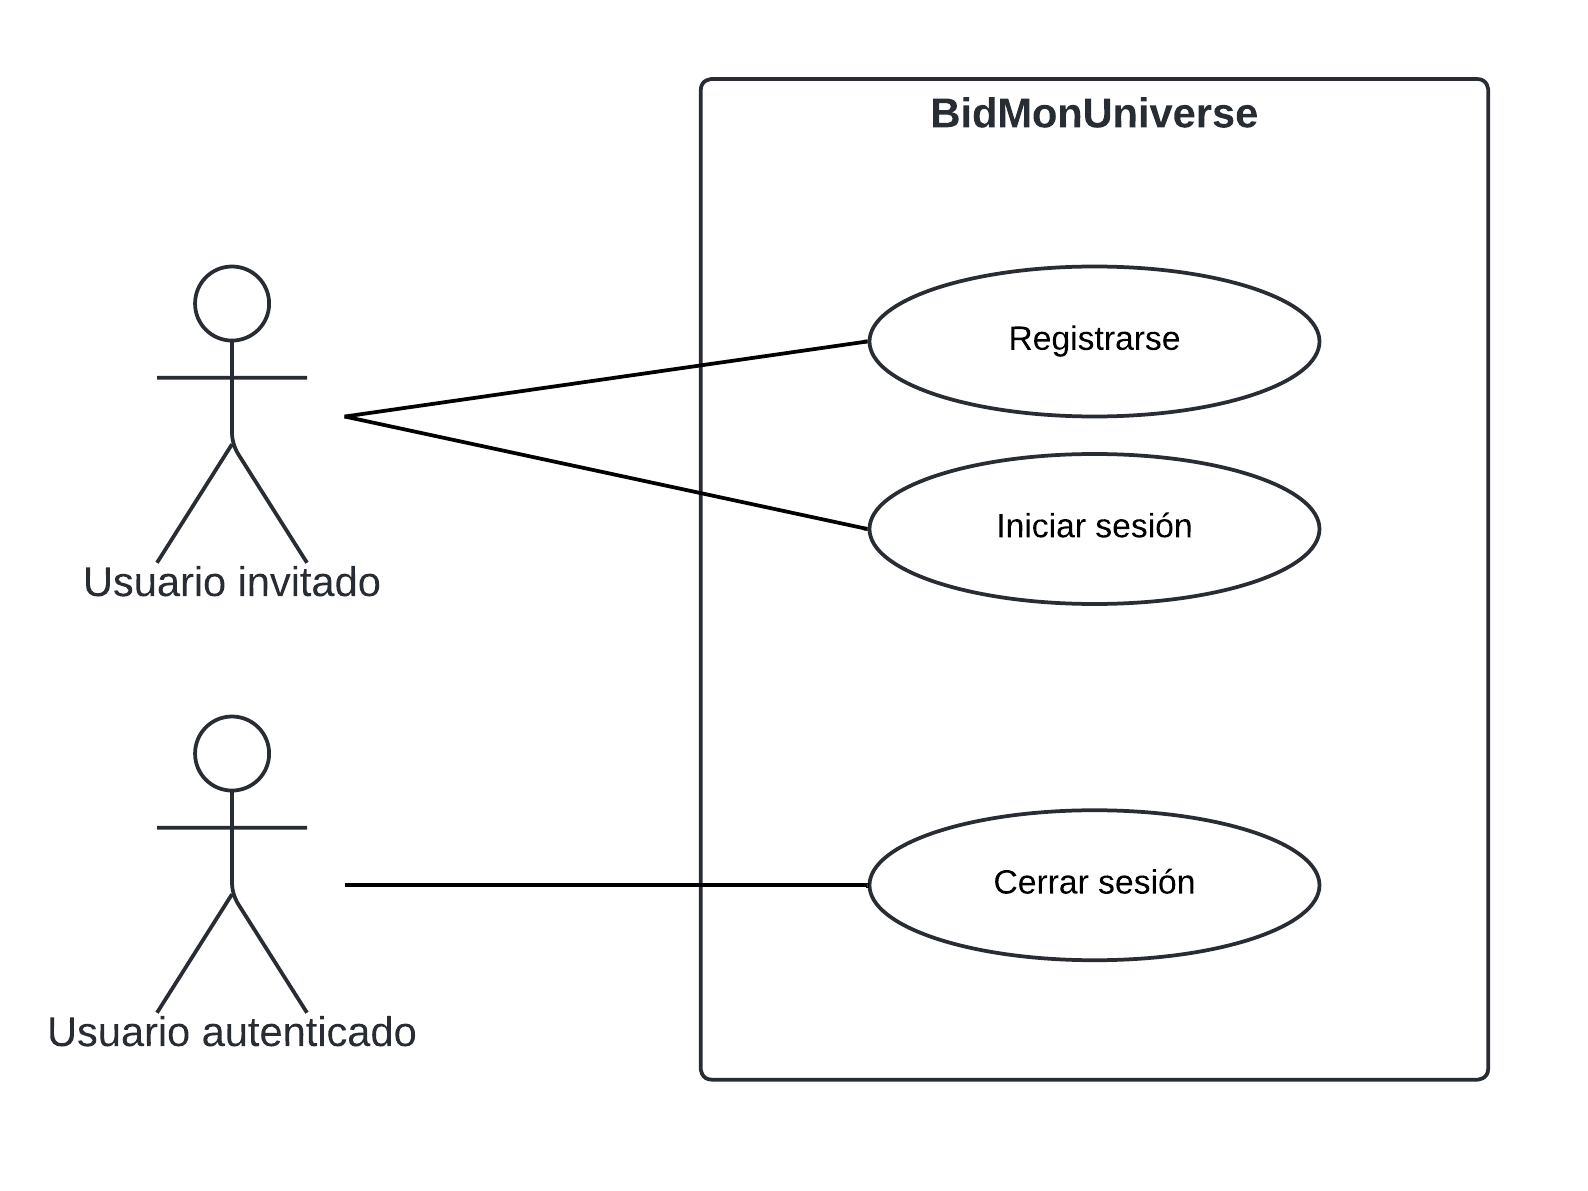
\includegraphics[width=0.5\textwidth]{figures/6-Analisis/6-Casos-uso/6_3_1_Registro-inicio-sesion.png}
    \caption{Casos de uso. Registrarse e iniciar sesión}
    \label{fig:cu_registro-inicio-sesion}
\end{figure}


\subsubsection{Caso de uso. Registrarse} \label{sec:cu_registro}
\begin{longtable}{
    >{\columncolor{lightgreen!20}}p{4cm}
    p{12cm}
    }
    \caption{Caso de uso. Registrarse} \label{table:cu_registro} \\
    \toprule
    \rowcolor{darkgreen!50}
    \textbf{Caso de uso} & \multicolumn{1}{>{\columncolor{darkgreen!50}\centering\arraybackslash}p{12cm}}{\textbf{REGISTRO}} \\
    \endfirsthead
    
    \multicolumn{2}{c}%
    {{ \tablename\ \thetable{} Caso de uso. Registrarse -- continuación de la página anterior}} \\
    \toprule
    \rowcolor{darkgreen!50}
    \textbf{Caso de uso} & \multicolumn{1}{>{\columncolor{darkgreen!50}\centering\arraybackslash}p{12cm}}{\textbf{REGISTRO}} \\
    \midrule
    \endhead
    
    \midrule
    \multicolumn{2}{r}{{Continúa en la siguiente página...}} \\ 
    \endfoot
    
    \bottomrule
    \endlastfoot
    
    \midrule
    Descripción & Un usuario no autenticado se puede registrar en el sistema para poder acceder a las funcionalidades del mismo. \\
    \midrule
    Actores principales & Usuario no autenticado \\
    \midrule
    Actores secundarios &  \\
    \midrule
    Precondiciones & El usuario no debe estar registrado en el sistema. \\
    \midrule
    Postcondiciones & \begin{itemize}[nosep,leftmargin=*]
      \item Se crea un nuevo registro en la base de datos con los datos del usuario.
      \item Se notifica al usuario que su registro ha sido exitoso.
      \item Se redirige al usuario a la página de inicio de sesión.
    \end{itemize} \\
    \midrule
    Disparadores & El usuario hace clic en el botón de registro. \\
    \midrule
    Escenario principal & \begin{enumerate}[nosep,leftmargin=*]
      \item El sistema muestra el formulario de registro.
      \item El usuario completa el formulario con sus datos personales.
      \item El usuario hace clic en el botón de registro.
      \item El sistema valida los datos del formulario.
      \item El sistema crea un nuevo registro en la base de datos con los datos del usuario.
      \item El sistema notifica al usuario que su registro ha sido exitoso.
      \item El sistema redirige al usuario a la página de inicio de sesión.
    \end{enumerate} \\
    \midrule
    Escenarios alternativos & 
    \begin{itemize}[nosep,leftmargin=*]
      \item \textbf{Escenario alternativo 1. El usuario cancela el registro.}
      \begin{enumerate}[nosep,leftmargin=*]
          \item El usuario hace clic en otro enlace.
          \item El sistema no crea el registro y redirige al usuario a la página correspondiente.
      \end{enumerate}
      \item \textbf{Escenario alternativo 2. El usuario ya está registrado en el sistema.}
      \begin{enumerate}[nosep,leftmargin=*]
          \item El sistema muestra un mensaje de error.
          \item El sistema no crea el registro y redirige al usuario de nuevo al formulario de registro.
      \end{enumerate}
      \item \textbf{Escenario alternativo 3. El usuario no completa el formulario correctamente.}
      \begin{enumerate}[nosep,leftmargin=*]
          \item El sistema muestra un mensaje de error con los campos que no se han completado correctamente.
          \item El sistema no crea el registro y redirige al usuario de nuevo al formulario de registro.
      \end{enumerate}
    \end{itemize} \\
    \midrule
    Situaciones de error & \begin{itemize}[nosep,leftmargin=*]
      \item \textbf{Error de conexión a la base de datos.}
      \begin{enumerate}[nosep,leftmargin=*]
          \item El sistema muestra un mensaje de error.
          \item El sistema redirige al usuario de nuevo al formulario de registro.
      \end{enumerate}
    \end{itemize} \\
    \end{longtable}


\subsubsection{Caso de uso. Iniciar sesión} \label{sec:cu_inicio-sesion}
\begin{longtable}{
    >{\columncolor{lightgreen!20}}p{4cm}
    p{12cm}
    }
    \caption{Caso de uso. Iniciar sesión} \label{table:cu_inicio-sesion} \\
    \toprule
    \rowcolor{darkgreen!50}
    \textbf{Caso de uso} & \multicolumn{1}{>{\columncolor{darkgreen!50}\centering\arraybackslash}p{12cm}}{\textbf{INICIAR SESIÓN}} \\
    \endfirsthead
    
    \multicolumn{2}{c}%
    {{ \tablename\ \thetable{} Caso de uso. Iniciar sesión -- continuación de la página anterior}} \\
    \toprule
    \rowcolor{darkgreen!50}
    \textbf{Caso de uso} & \multicolumn{1}{>{\columncolor{darkgreen!50}\centering\arraybackslash}p{12cm}}{\textbf{INICIAR SESIÓN}} \\
    \midrule
    \endhead
    
    \midrule
    \multicolumn{2}{r}{{Continúa en la siguiente página...}} \\ 
    \endfoot
    
    \bottomrule
    \endlastfoot
    
    \midrule
    Descripción & Un usuario no autenticado puede iniciar sesión en el sistema para acceder a las funcionalidades del mismo. \\
    \midrule
    Actores principales & Usuario no autenticado \\
    \midrule
    Actores secundarios &  \\
    \midrule
    Precondiciones & El usuario debe de haberse registrado previamente en el sistema. \\
    \midrule
    Postcondiciones & \begin{itemize}[nosep,leftmargin=*]
        \item Se crea una nueva sesión para el usuario.
        \item Se redirige al usuario a la página de inicio.
    \end{itemize} \\
    \midrule
    Disparadores & El usuario hace clic en el botón de inicio de sesión. \\
    \midrule
    Escenario principal & \begin{enumerate}[nosep,leftmargin=*]
        \item El sistema muestra el formulario de inicio de sesión.
        \item El usuario completa el formulario con sus credenciales.
        \item El usuario hace clic en el botón de inicio de sesión.
        \item El sistema valida las credenciales del usuario.
        \item El sistema crea una nueva sesión para el usuario.
        \item El sistema redirige al usuario a la página de inicio.
    \end{enumerate} \\
    \midrule
    Escenarios alternativos & 
    \begin{itemize}[nosep,leftmargin=*]
      \item \textbf{Escenario alternativo 1. El usuario cancela el inicio de sesión.}
      \begin{enumerate}[nosep,leftmargin=*]
          \item El usuario hace clic en otro enlace.
          \item El sistema no crea la sesión para el usuario y redirige al usuario a la página correspondiente.
      \end{enumerate}
      \item \textbf{Escenario alternativo 2. El usuario no está registrado en el sistema o la contraseña es incorrecta.}
      \begin{enumerate}[nosep,leftmargin=*]
          \item El sistema muestra un mensaje de error.
          \item El sistema no crea la sesión para el usuario y redirige al usuario de nuevo al formulario de inicio de sesión.
      \end{enumerate}
      \item \textbf{Escenario alternativo 3. El usuario no completa el formulario correctamente.}
      \begin{enumerate}[nosep,leftmargin=*]
          \item El sistema muestra un mensaje de error con los campos que no se han completado correctamente.
          \item El sistema no crea la sesión para el usuario y redirige al usuario de nuevo al formulario de inicio de sesión.
      \end{enumerate}
    \end{itemize} \\
    \midrule
    Situaciones de error & \begin{itemize}[nosep,leftmargin=*]
      \item \textbf{Error de conexión a la base de datos.}
      \begin{enumerate}[nosep,leftmargin=*]
          \item El sistema muestra un mensaje de error.
          \item El sistema redirige al usuario de nuevo al formulario de inicio de sesión.
      \end{enumerate}
    \end{itemize} \\
    \end{longtable}


\subsubsection{Caso de uso. Cerrar sesión} \label{sec:cu_cerrar-sesion}
\begin{longtable}{
    >{\columncolor{lightgreen!20}}p{4cm}
    p{12cm}
    }
    \caption{Caso de uso. Cerrar sesión} \label{table:cu_cerrar-sesion} \\
    \toprule
    \rowcolor{darkgreen!50}
    \textbf{Caso de uso} & \multicolumn{1}{>{\columncolor{darkgreen!50}\centering\arraybackslash}p{12cm}}{\textbf{CERRAR SESIÓN}} \\
    \endfirsthead
    
    \multicolumn{2}{c}%
    {{ \tablename\ \thetable{} Caso de uso. Cerrar sesión -- continuación de la página anterior}} \\
    \toprule
    \rowcolor{darkgreen!50}
    \textbf{Caso de uso} & \multicolumn{1}{>{\columncolor{darkgreen!50}\centering\arraybackslash}p{12cm}}{\textbf{CERRAR SESIÓN}} \\
    \midrule
    \endhead
    
    \midrule
    \multicolumn{2}{r}{{Continúa en la siguiente página...}} \\ 
    \endfoot
    
    \bottomrule
    \endlastfoot
    
    \midrule
    Descripción & Un usuario autenticado puede cerrar sesión en el sistema. \\
    \midrule
    Actores principales & Usuario autenticado \\
    \midrule
    Actores secundarios &  \\
    \midrule
    Precondiciones & El usuario debe de haber iniciado sesión previamente en el sistema. \\
    \midrule
    Postcondiciones & \begin{itemize}[nosep,leftmargin=*]
        \item Se elimina la sesión del usuario.
    \end{itemize} \\
    \midrule
    Disparadores & El usuario hace clic en el botón de cerrar sesión. \\
    \midrule
    Escenario principal & \begin{enumerate}[nosep,leftmargin=*]
        \item El sistema muestra la opción de cerrar sesión.
        \item El usuario hace clic en el botón de cerrar sesión.
        \item El sistema elimina la sesión del usuario.
        \item El sistema redirige al usuario a la página de inicio.
    \end{enumerate} \\
    \midrule
    Escenarios alternativos & \\
    \midrule
    Situaciones de error & \\
    \end{longtable}

\newpage
\subsection{Casos de uso. Gestión de perfil}
\begin{figure}[H]
    \centering
    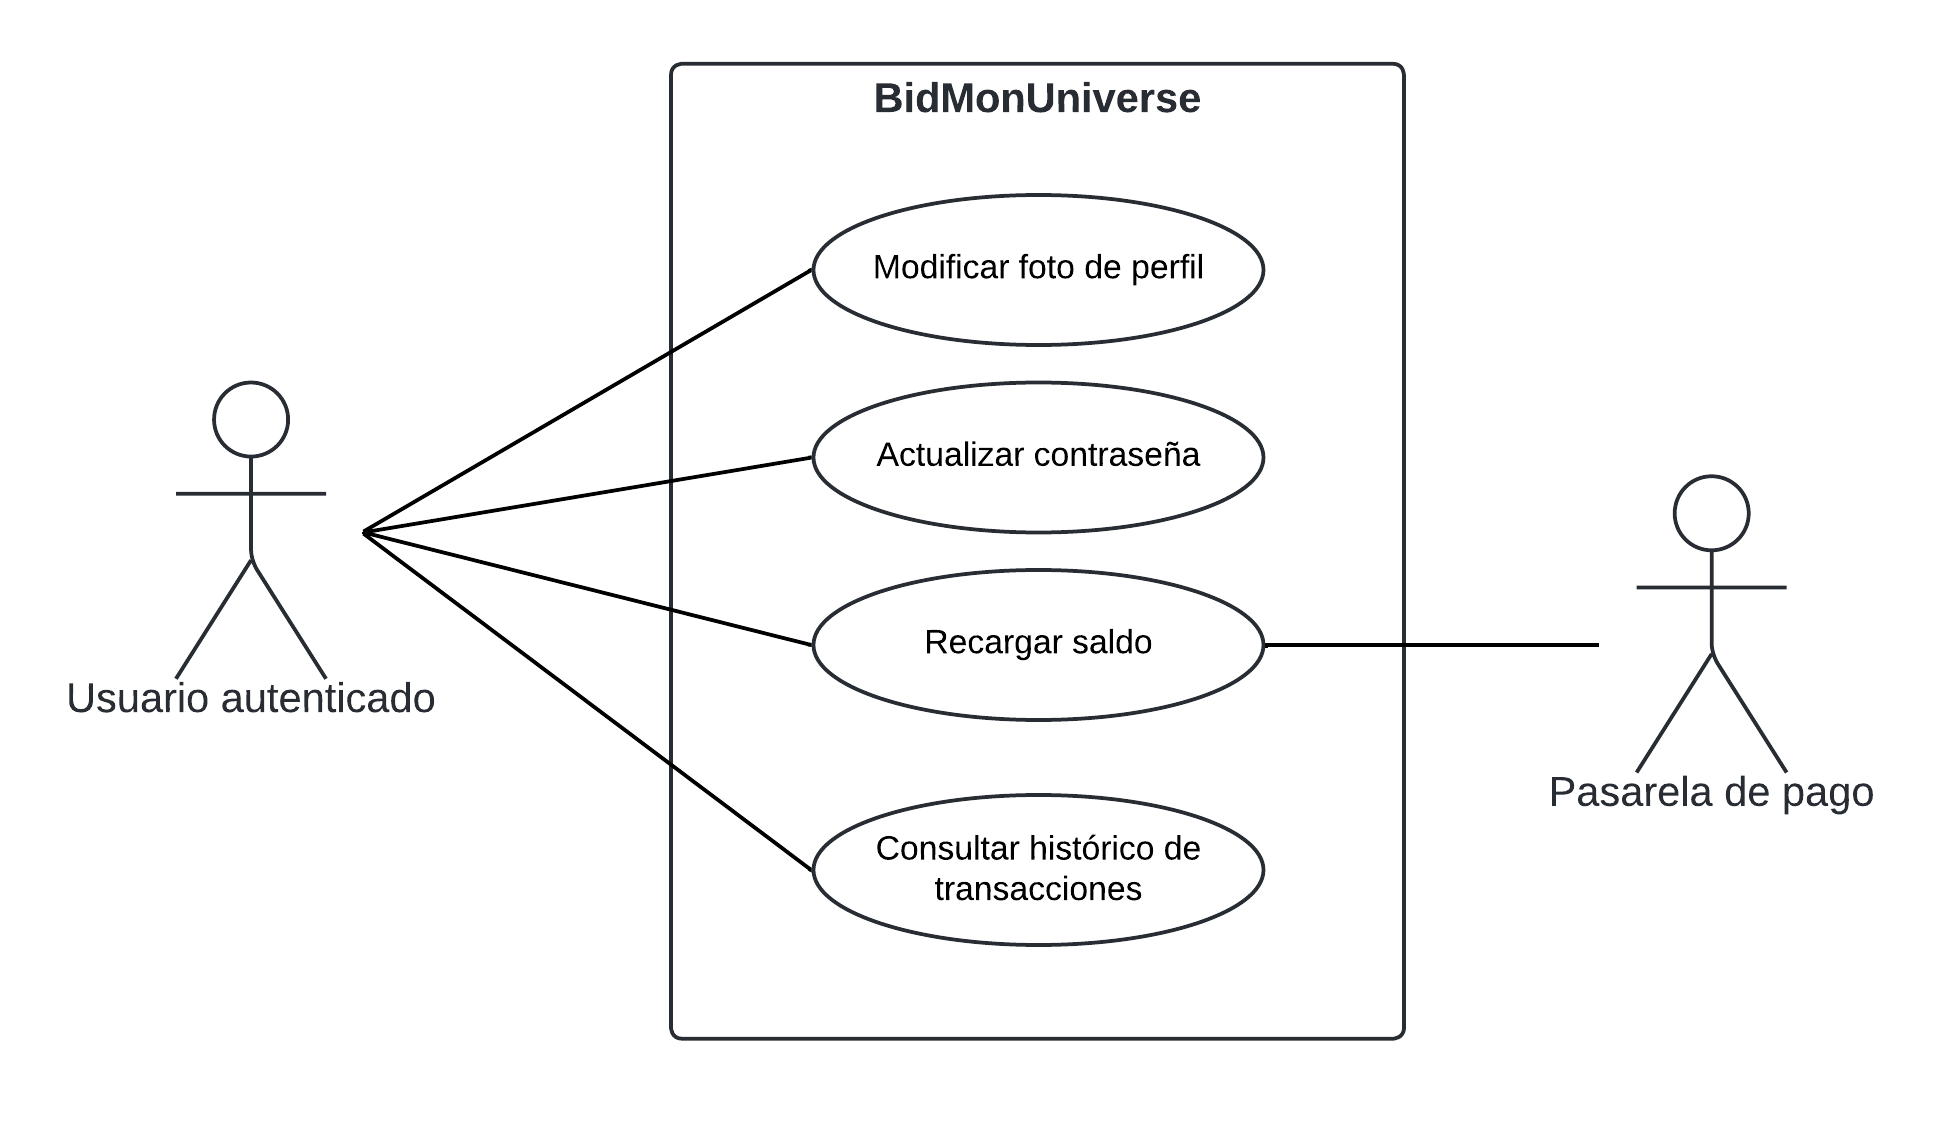
\includegraphics[width=0.5\textwidth]{figures/6-Analisis/6-Casos-uso/6_3_2_Gestion-perfil.png}
    \caption{Casos de uso. Gestión de perfil}
    \label{fig:cu_gestion-perfil}
\end{figure}
\subsubsection{Caso de uso. Modificar foto de perfil} \label{sec:cu_modificar-perfil}
\begin{longtable}{
    >{\columncolor{lightgreen!20}}p{4cm}
    p{12cm}
    }
    \caption{Caso de uso. Modificar foto de perfil} \label{table:cu_modificar-perfil} \\
    \toprule
    \rowcolor{darkgreen!50}
    \textbf{Caso de uso} & \multicolumn{1}{>{\columncolor{darkgreen!50}\centering\arraybackslash}p{12cm}}{\textbf{MODIFICAR PERFIL}} \\
    \endfirsthead
    
    \multicolumn{2}{c}%
    {{ \tablename\ \thetable{} Caso de uso. Modificar foto de perfil -- continuación de la página anterior}} \\
    \toprule
    \rowcolor{darkgreen!50}
    \textbf{Caso de uso} & \multicolumn{1}{>{\columncolor{darkgreen!50}\centering\arraybackslash}p{12cm}}{\textbf{MODIFICAR PERFIL}} \\
    \midrule
    \endhead
    
    \midrule
    \multicolumn{2}{r}{{Continúa en la siguiente página...}} \\ 
    \endfoot
    
    \bottomrule
    \endlastfoot
    
    \midrule
    Descripción & Un usuario autenticado puede modificar su foto de perfil de usuario. \\
    \midrule
    Actores principales & Usuario autenticado \\
    \midrule
    Actores secundarios &  \\
    \midrule
    Precondiciones & \begin{itemize}[nosep,leftmargin=*]
        \item El usuario debe haber iniciado sesión en el sistema.
    \end{itemize} \\
    \midrule
    Postcondiciones & \begin{itemize}[nosep,leftmargin=*]
        \item Se modifica el campo de la foto de perfil del usuario en la base de datos.
    \end{itemize} \\
    \midrule
    Disparadores & El usuario accede a la sección de modificar perfil. \\
    \midrule
    Escenario principal & \begin{enumerate}[nosep,leftmargin=*]
        \item El usuario accede a la sección de modificar perfil.
        \item El sistema muestra la opción de modificar la foto de perfil.
        \item El usuario hace clic en la opción de modificar la foto de perfil.
        \item El sistema muestra las imágenes predefinidas para que el usuario pueda seleccionar una.
        \item El usuario selecciona una imagen.
        \item El usuario hace clic en el botón de guardar.
        \item El sistema modifica el campo de la foto de perfil del usuario en la base de datos.
        \item El sistema muestra un mensaje de éxito.
        \item El sistema redirige al usuario a la página principal.
    \end{enumerate} \\
    \midrule
    Escenarios alternativos & 
    \begin{itemize}[nosep,leftmargin=*]
        \item \textbf{Escenario alternativo 1. El usuario cancela la modificación de perfil.}
        \begin{enumerate}[nosep,leftmargin=*]
            \item El usuario no hace clic en el botón de guardar.
            \item El sistema no modifica los datos del perfil del usuario.
        \end{enumerate}
    \end{itemize} \\
    \midrule
    Situaciones de error & 
    \begin{itemize}[nosep,leftmargin=*]
        \item \textbf{Error de conexión a la base de datos.}
        \begin{enumerate}[nosep,leftmargin=*]
            \item El sistema mostrará un mensaje de error.
            \item El sistema no modificará los datos del perfil del usuario.
        \end{enumerate}
    \end{itemize} \\
\end{longtable}


\subsubsection{Caso de uso. Actualizar contraseña} \label{sec:cu_actualizar-contrasena}
\begin{longtable}{
    >{\columncolor{lightgreen!20}}p{4cm}
    p{12cm}
    }
    \caption{Caso de uso. Actualizar contraseña} \label{table:cu_actualizar-contrasena} \\
    \toprule
    \rowcolor{darkgreen!50}
    \textbf{Caso de uso} & \multicolumn{1}{>{\columncolor{darkgreen!50}\centering\arraybackslash}p{12cm}}{\textbf{ACTUALIZAR CONTRASEÑA}} \\
    \endfirsthead
    
    \multicolumn{2}{c}%
    {{ \tablename\ \thetable{} Caso de uso. Actualizar contraseña -- continuación de la página anterior}} \\
    \toprule
    \rowcolor{darkgreen!50}
    \textbf{Caso de uso} & \multicolumn{1}{>{\columncolor{darkgreen!50}\centering\arraybackslash}p{12cm}}{\textbf{ACTUALIZAR CONTRASEÑA}} \\
    \midrule
    \endhead
    
    \midrule
    \multicolumn{2}{r}{{Continúa en la siguiente página...}} \\ 
    \endfoot
    
    \bottomrule
    \endlastfoot
    
    \midrule
    Descripción & Un usuario autenticado puede actualizar su contraseña de usuario. \\
    \midrule
    Actores principales & Usuario autenticado \\
    \midrule
    Actores secundarios &  \\
    \midrule
    Precondiciones & \begin{itemize}[nosep,leftmargin=*]
        \item El usuario debe haber iniciado sesión en el sistema.
    \end{itemize} \\
    \midrule
    Postcondiciones & \begin{itemize}[nosep,leftmargin=*]
        \item Se modifica la contraseña del usuario en la base de datos.
    \end{itemize} \\
    \midrule
    Disparadores & El usuario accede a la sección de modificar perfil. \\
    \midrule
    Escenario principal & \begin{enumerate}[nosep,leftmargin=*]
        \item El usuario accede a la sección de modificar perfil.
        \item El sistema muestra la opción de modificar la contraseña.
        \item El usuario hace clic en la opción de modificar la contraseña.
        \item El sistema muestra un formulario con los campos de la nueva contraseña y la confirmación de la nueva contraseña.
        \item El usuario completa los campos del formulario.
        \item El usuario hace clic en el botón de guardar.
        \item El sistema modifica el campo de la contraseña del usuario en la base de datos.
        \item El sistema muestra un mensaje de éxito.
        \item El sistema redirige al usuario a la página principal.
    \end{enumerate} \\
    \midrule
    Escenarios alternativos & 
    \begin{itemize}[nosep,leftmargin=*]
        \item \textbf{Escenario alternativo 1. El usuario cancela la modificación de perfil.}
        \begin{enumerate}[nosep,leftmargin=*]
            \item El usuario no hace clic en el botón de guardar.
            \item El sistema no modifica los datos del perfil del usuario.
        \end{enumerate}
        \item \textbf{Escenario alternativo 2. El usuario no completa correctamente los campos del formulario.}
        \begin{enumerate}[nosep,leftmargin=*]
            \item El usuario no completa correctamente los campos del formulario.
            \item El sistema muestra un mensaje de error.
            \item El sistema no modifica los datos del perfil del usuario.
        \end{enumerate}
    \end{itemize} \\
    \midrule
    Situaciones de error & 
    \begin{itemize}[nosep,leftmargin=*]
        \item \textbf{Error de conexión a la base de datos.}
        \begin{enumerate}[nosep,leftmargin=*]
            \item El sistema mostrará un mensaje de error.
            \item El sistema no modificará los datos del perfil del usuario.
        \end{enumerate}
    \end{itemize} \\
\end{longtable}




\subsubsection{Caso de uso. Recargar saldo} \label{sec:cu_recarga-saldo}
\begin{longtable}{
    >{\columncolor{lightgreen!20}}p{4cm}
    p{12cm}
    }
    \caption{Caso de uso. Recargar saldo} \label{table:cu_recarga-saldo} \\
    \toprule
    \rowcolor{darkgreen!50}
    \textbf{Caso de uso} & \multicolumn{1}{>{\columncolor{darkgreen!50}\centering\arraybackslash}p{12cm}}{\textbf{RECRAGAR SALDO}} \\
    \endfirsthead
    
    \multicolumn{2}{c}%
    {{ \tablename\ \thetable{} Caso de uso. Recargar saldo -- continuación de la página anterior}} \\
    \toprule
    \rowcolor{darkgreen!50}
    \textbf{Caso de uso} & \multicolumn{1}{>{\columncolor{darkgreen!50}\centering\arraybackslash}p{12cm}}{\textbf{RECARGAR SALDO}} \\
    \midrule
    \endhead
    
    \midrule
    \multicolumn{2}{r}{{Continúa en la siguiente página...}} \\ 
    \endfoot
    
    \bottomrule
    \endlastfoot
    
    \midrule
    Descripción & Un usuario autenticado puede recargar saldo en su cuenta. \\
    \midrule
    Actores principales & Usuario autenticado \\
    \midrule
    Actores secundarios &  Pasarela de pago \\
    \midrule
    Precondiciones & \begin{itemize}[nosep,leftmargin=*]
        \item El usuario debe haber iniciado sesión en el sistema.
    \end{itemize} \\
    \midrule
    Postcondiciones & \begin{itemize}[nosep,leftmargin=*]
        \item Se incrementa el saldo del usuario en la base de datos.
    \end{itemize} \\
    \midrule
    Disparadores & El usuario accede a la sección de recarga de saldo. \\
    \midrule
    Escenario principal & \begin{enumerate}[nosep,leftmargin=*]
        \item El sistema muestra el formulario de recarga de saldo.
        \item El usuario introduce la cantidad de saldo que desea recargar.
        \item El usuario hace clic en el botón de recargar saldo.
        \item El sistema valida la cantidad de saldo introducida.
        \item El sistema redirige al usuario a la pasarela de pago.
        \item El usuario completa el pago.
        \item El sistema incrementa el saldo del usuario en la base de datos.
        \item El sistema muestra un mensaje de éxito.
    \end{enumerate} \\
    \midrule
    Escenarios alternativos & 
    \begin{itemize}[nosep,leftmargin=*]
        \item \textbf{Escenario alternativo 1. El usuario cancela la recarga de saldo en la pasarela de pago.}
        \begin{enumerate}[nosep,leftmargin=*]
            \item El usuario cancela el pago.
            \item El sistema no incrementa el saldo del usuario en la base de datos.
            \item El sistema redirige al usuario a la página que muestra su saldo actual.
            \item El sistema muestra un mensaje de cancelación.
        \end{enumerate}
        \item \textbf{Escenario alternativo 2. El usuario introduce una cantidad de saldo inválida.}
        \begin{enumerate}[nosep,leftmargin=*]
            \item El sistema muestra un mensaje de error.
            \item El sistema muestra los campos con errores.
            \item El sistema permite al usuario corregir los errores.
        \end{enumerate}
    \end{itemize} \\
    \midrule
    Situaciones de error & 
    \begin{itemize}[nosep,leftmargin=*]
        \item \textbf{Error de conexión a la base de datos.}
        \begin{enumerate}[nosep,leftmargin=*]
            \item El sistema mostrará un mensaje de error.
            \item El sistema no incrementará el saldo del usuario en la base de datos.
            \item El sistema le dará al usuario la opción de intentar recargar de nuevo el saldo o volver a la página de inicio.
        \end{enumerate}
        \item \textbf{Error en la pasarela de pago.}
        \begin{enumerate}[nosep,leftmargin=*]
            \item El sistema mostrará un mensaje de error.
            \item El sistema no incrementará el saldo del usuario en la base de datos.
            \item El sistema redirigirá al usuario a la página de recarga de saldo.
        \end{enumerate}
    \end{itemize} \\
\end{longtable}

\subsubsection{Caso de uso. Histórico de transacciones realizadas} \label{sec:cu_transacciones-realizadas}
\begin{longtable}{
    >{\columncolor{lightgreen!20}}p{4cm}
    >{\columncolor{white}}p{12cm} 
    }
    \caption{Caso de uso. Histórico de transacciones realizadas} \label{table:cu_transacciones-realizadas} \\
    \toprule
    \rowcolor{darkgreen!50}
    \textbf{Caso de uso} & \multicolumn{1}{>{\columncolor{darkgreen!50}\centering\arraybackslash}p{12cm}}{\textbf{HISTÓRICO DE TRANSACCIONES REALIZADAS}} \\
    \endfirsthead
    
    \multicolumn{2}{c}%
    {{ \tablename\ \thetable{} Caso de uso. Histórico de transacciones realizadas -- continuación de la página anterior}} \\
    \toprule
    \rowcolor{darkgreen!50}
    \textbf{Caso de uso} & \multicolumn{1}{>{\columncolor{darkgreen!50}\centering\arraybackslash}p{12cm}}{\textbf{HISTÓRICO DE TRANSACCIONES REALIZADAS}} \\
    \midrule
    \endhead
    
    \midrule
    \multicolumn{2}{r}{{Continúa en la siguiente página...}} \\ 
    \endfoot
    
    \bottomrule
    \endlastfoot
    
    \midrule
    Descripción & Un usuario autenticado puede consultar el histórico de transacciones realizadas en el sistema. \\
    \midrule
    Actores principales & Usuario autenticado \\
    \midrule
    Actores secundarios &  \\
    \midrule
    Precondiciones & \begin{itemize}[nosep,leftmargin=*]
        \item El usuario debe haber iniciado sesión en el sistema.
    \end{itemize} \\
    \midrule
    Postcondiciones & \\
    \midrule
    Disparadores & El usuario accede a la sección de historial de transacciones. \\
    \midrule
    Escenario principal & \begin{enumerate}[nosep,leftmargin=*]
        \item El sistema muestra el historial de transacciones del usuario.
    \end{enumerate} \\
    \midrule
    Escenarios alternativos & 
    \begin{itemize}[nosep,leftmargin=*]
        \item \textbf{Escenario alternativo 1. El usuario no tiene transacciones realizadas.}
        \begin{enumerate}[nosep,leftmargin=*]
            \item El sistema mostrará un mensaje indicando que el usuario no tiene transacciones realizadas.
        \end{enumerate}
    \end{itemize} \\
    \midrule
    Situaciones de error & 
    \begin{itemize}[nosep,leftmargin=*]
        \item \textbf{Error de conexión a la base de datos.}
        \begin{enumerate}[nosep,leftmargin=*]
            \item El sistema mostrará un mensaje de error.
            \item El sistema le dará al usuario la opción de intentar cargar de nuevo el historial de transacciones o volver a la página principal.
        \end{enumerate}
    \end{itemize} \\
\end{longtable}

\newpage
\subsection{Casos de uso. Gestión de colección de cartas}
\begin{figure}[H]
    \centering
    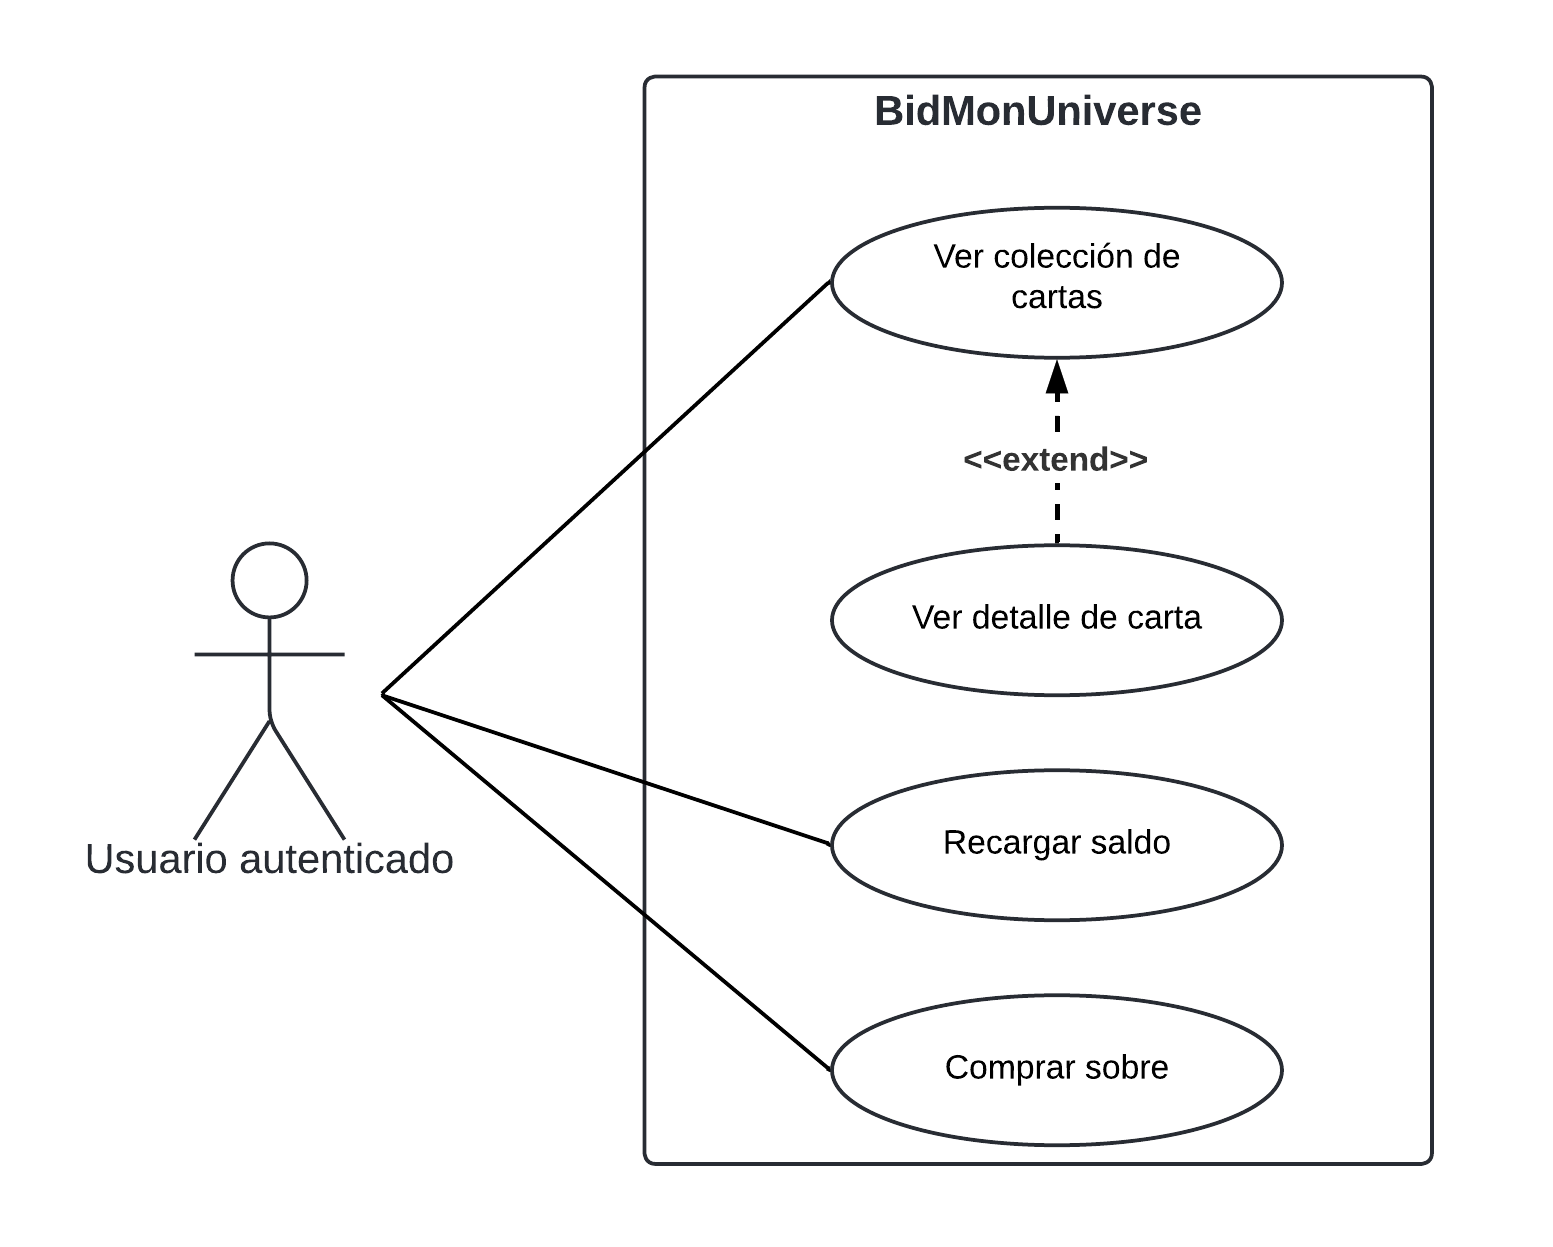
\includegraphics[width=0.5\textwidth]{figures/6-Analisis/6-Casos-uso/6_3_3_Gestion-coleccion-cartas.png}
    \caption{Casos de uso. Gestión de colección de cartas}
    \label{fig:cu_gestion-coleccion-cartas}
\end{figure}

\subsubsection{Caso de uso. Ver colección de cartas} \label{sec:cu_coleccion-cartas}
\begin{longtable}{
    >{\columncolor{lightgreen!20}}p{4cm}
    p{12cm}
    }
    \caption{Caso de uso. Ver colección de cartas} \label{table:cu_coleccion-cartas} \\
    \toprule
    \rowcolor{darkgreen!50}
    \textbf{Caso de uso} & \multicolumn{1}{>{\columncolor{darkgreen!50}\centering\arraybackslash}p{12cm}}{\textbf{VER COLECCIÓN DE CARTAS}} \\
    \endfirsthead
    
    \multicolumn{2}{c}%
    {{ \tablename\ \thetable{} Caso de uso. Ver colección de cartas -- continuación de la página anterior}} \\
    \toprule
    \rowcolor{darkgreen!50}
    \textbf{Caso de uso} & \multicolumn{1}{>{\columncolor{darkgreen!50}\centering\arraybackslash}p{12cm}}{\textbf{VER COLECCIÓN DE CARTAS}} \\
    \midrule
    \endhead
    
    \midrule
    \multicolumn{2}{r}{{Continúa en la siguiente página...}} \\ 
    \endfoot
    
    \bottomrule
    \endlastfoot
    
    \midrule
    Descripción & Un usuario autenticado puede ver la colección de cartas que posee. \\
    \midrule
    Actores principales & Usuario autenticado \\
    \midrule
    Actores secundarios &  \\
    \midrule
    Precondiciones & \begin{itemize}[nosep,leftmargin=*]
        \item El usuario debe haber iniciado sesión en el sistema.
    \end{itemize} \\
    \midrule
    Postcondiciones & \\
    \midrule
    Disparadores & El usuario accede a la sección de colección de cartas. \\
    \midrule
    Escenario principal & \begin{enumerate}[nosep,leftmargin=*]
        \item El sistema muestra la colección de cartas del usuario.
    \end{enumerate} \\
    \midrule
    Escenarios alternativos & 
    \begin{itemize}[nosep,leftmargin=*]
        \item \textbf{Escenario alternativo 1. El usuario no tiene cartas en su colección.}
        \begin{enumerate}[nosep,leftmargin=*]
            \item Se mostrará un mensaje indicando que el usuario no tiene cartas en su colección.
            \item Se mostrará la opción de comprar un sobre de cartas.
        \end{enumerate}
    \end{itemize} \\
    \midrule
    Situaciones de error & 
    \begin{itemize}[nosep,leftmargin=*]
        \item \textbf{Error de conexión a la base de datos.}
        \begin{enumerate}[nosep,leftmargin=*]
            \item El sistema mostrará un mensaje de error.
            \item El sistema le dará al usuario la opción de volver a la página principal.
        \end{enumerate}
    \end{itemize} \\
\end{longtable}

\subsubsection{Caso de uso. Ver detalle de una carta} \label{sec:cu_detalle-carta}
\begin{longtable}{
    >{\columncolor{lightgreen!20}}p{4cm}
    p{12cm}
    }
    \caption{Caso de uso. Ver detalle de una carta} \label{table:cu_detalle-carta} \\
    \toprule
    \rowcolor{darkgreen!50}
    \textbf{Caso de uso} & \multicolumn{1}{>{\columncolor{darkgreen!50}\centering\arraybackslash}p{12cm}}{\textbf{VER DETALLE DE UNA CARTA}} \\
    \endfirsthead
    
    \multicolumn{2}{c}%
    {{ \tablename\ \thetable{} Caso de uso. Ver detalle de una carta -- continuación de la página anterior}} \\
    \toprule
    \rowcolor{darkgreen!50}
    \textbf{Caso de uso} & \multicolumn{1}{>{\columncolor{darkgreen!50}\centering\arraybackslash}p{12cm}}{\textbf{VER DETALLE DE UNA CARTA}} \\
    \midrule
    \endhead
    
    \midrule
    \multicolumn{2}{r}{{Continúa en la siguiente página...}} \\ 
    \endfoot
    
    \bottomrule
    \endlastfoot
    
    \midrule
    Descripción & Un usuario autenticado puede ver el detalle de una carta de su colección. \\
    \midrule
    Actores principales & Usuario autenticado \\
    \midrule
    Actores secundarios &  \\
    \midrule
    Precondiciones & \begin{itemize}[nosep,leftmargin=*]
        \item El usuario debe haber iniciado sesión en el sistema.
    \end{itemize} \\
    \midrule
    Postcondiciones & \\
    \midrule
    Disparadores & El usuario accede a la sección de colección de cartas y selecciona una carta. \\
    \midrule
    Escenario principal & \begin{enumerate}[nosep,leftmargin=*]
        \item El sistema muestra la colección de cartas del usuario.
        \item El usuario puede seleccionar una carta para ver su información detallada.
        \item El sistema redirige al usuario a la página de detalle de la carta seleccionada.
        \item El usuario puede consultar la información detallada de la carta.
        \item El usuario puede consultar el histórico de transacciones de la carta.
        \item Si la carta no está en subasta, el usuario puede ponerla en subasta.
    \end{enumerate} \\
    \midrule
    Escenarios alternativos &  \\
    \midrule
    Situaciones de error & 
    \begin{itemize}[nosep,leftmargin=*]
        \item \textbf{Error de conexión a la base de datos.}
        \begin{enumerate}[nosep,leftmargin=*]
            \item El sistema mostrará un mensaje de error.
            \item El sistema le dará al usuario la opción de volver a la página principal.
        \end{enumerate}
    \end{itemize} \\
\end{longtable}


\subsubsection{Caso de uso. Comprar sobre} \label{sec:cu_comprar-sobre}
\begin{longtable}{
    >{\columncolor{lightgreen!20}}p{4cm}
    p{12cm}
    }
    \caption{Caso de uso. Comprar sobre} \label{table:cu_comprar-sobre} \\
    \toprule
    \rowcolor{darkgreen!50}
    \textbf{Caso de uso} & \multicolumn{1}{>{\columncolor{darkgreen!50}\centering\arraybackslash}p{12cm}}{\textbf{COMPRAR SOBRE}} \\
    \endfirsthead
    
    \multicolumn{2}{c}%
    {{ \tablename\ \thetable{} Caso de uso. Comprar sobre -- continuación de la página anterior}} \\
    \toprule
    \rowcolor{darkgreen!50}
    \textbf{Caso de uso} & \multicolumn{1}{>{\columncolor{darkgreen!50}\centering\arraybackslash}p{12cm}}{\textbf{COMPRAR SOBRE}} \\
    \midrule
    \endhead
    
    \midrule
    \multicolumn{2}{r}{{Continúa en la siguiente página...}} \\ 
    \endfoot
    
    \bottomrule
    \endlastfoot
    
    \midrule
    Descripción & Un usuario autenticado puede comprar un sobre de cartas. \\
    \midrule
    Actores principales & Usuario autenticado \\
    \midrule
    Actores secundarios &  \\
    \midrule
    Precondiciones & \begin{itemize}[nosep,leftmargin=*]
        \item El usuario ha iniciado sesión en el sistema.
        \item El usuario dispone de saldo suficiente para comprar el sobre.
    \end{itemize} \\
    \midrule
    Postcondiciones & \begin{itemize}[nosep,leftmargin=*]
        \item Se descuenta el precio del sobre del saldo del usuario.
        \item Se añaden las cartas del sobre a la colección del usuario.
        \item Se decrementa en una unidad la cantidad de sobres disponibles en el inventario.
        \item Se registra la transacción en el historial de compras del usuario.
    \end{itemize} \\
    \midrule
    Disparadores & El usuario hace clic en el botón de comprar sobre. \\
    \midrule
    Escenario principal & \begin{enumerate}[nosep,leftmargin=*]
        \item El sistema muestra el inventario de sobres disponibles.
        \item El usuario selecciona el sobre que desea comprar.
        \item El usuario hace clic en el botón de comprar sobre.
        \item El sistema valida que el usuario dispone de saldo suficiente.
        \item El sistema descuenta el precio del sobre del saldo del usuario.
        \item El sistema genera las cartas del sobre.
        \item El sistema añade las cartas del sobre a la colección del usuario.
    \end{enumerate} \\
    \midrule
    Escenarios alternativos & 
    \begin{itemize}[nosep,leftmargin=*]
        \item \textbf{Escenario alternativo 1. El usuario intenta comprar un sobre sin saldo suficiente.}
        \begin{enumerate}[nosep,leftmargin=*]
            \item El usuario intenta comprar un sobre sin saldo suficiente.
            \item El sistema muestra un mensaje de error.
            \item El sistema le ofrece al usuario la posibilidad de recargar saldo.
        \end{enumerate}
    \end{itemize} \\
    \midrule
    Situaciones de error & 
    \begin{itemize}[nosep,leftmargin=*]
        \item \textbf{Error de conexión a la base de datos.}
        \begin{enumerate}[nosep,leftmargin=*]
            \item El sistema muestra un mensaje de error.
            \item El sistema no descuenta el precio del sobre del saldo del usuario.
            \item El sistema no añade las cartas del sobre a la colección del usuario.
            \item El sistema no decrementa en una unidad la cantidad de sobres disponibles en el inventario.
        \end{enumerate}
    \end{itemize} \\
\end{longtable}



\newpage
\subsection{Casos de uso. Gestión de subastas y pujas}
\begin{figure}[H]
    \centering
    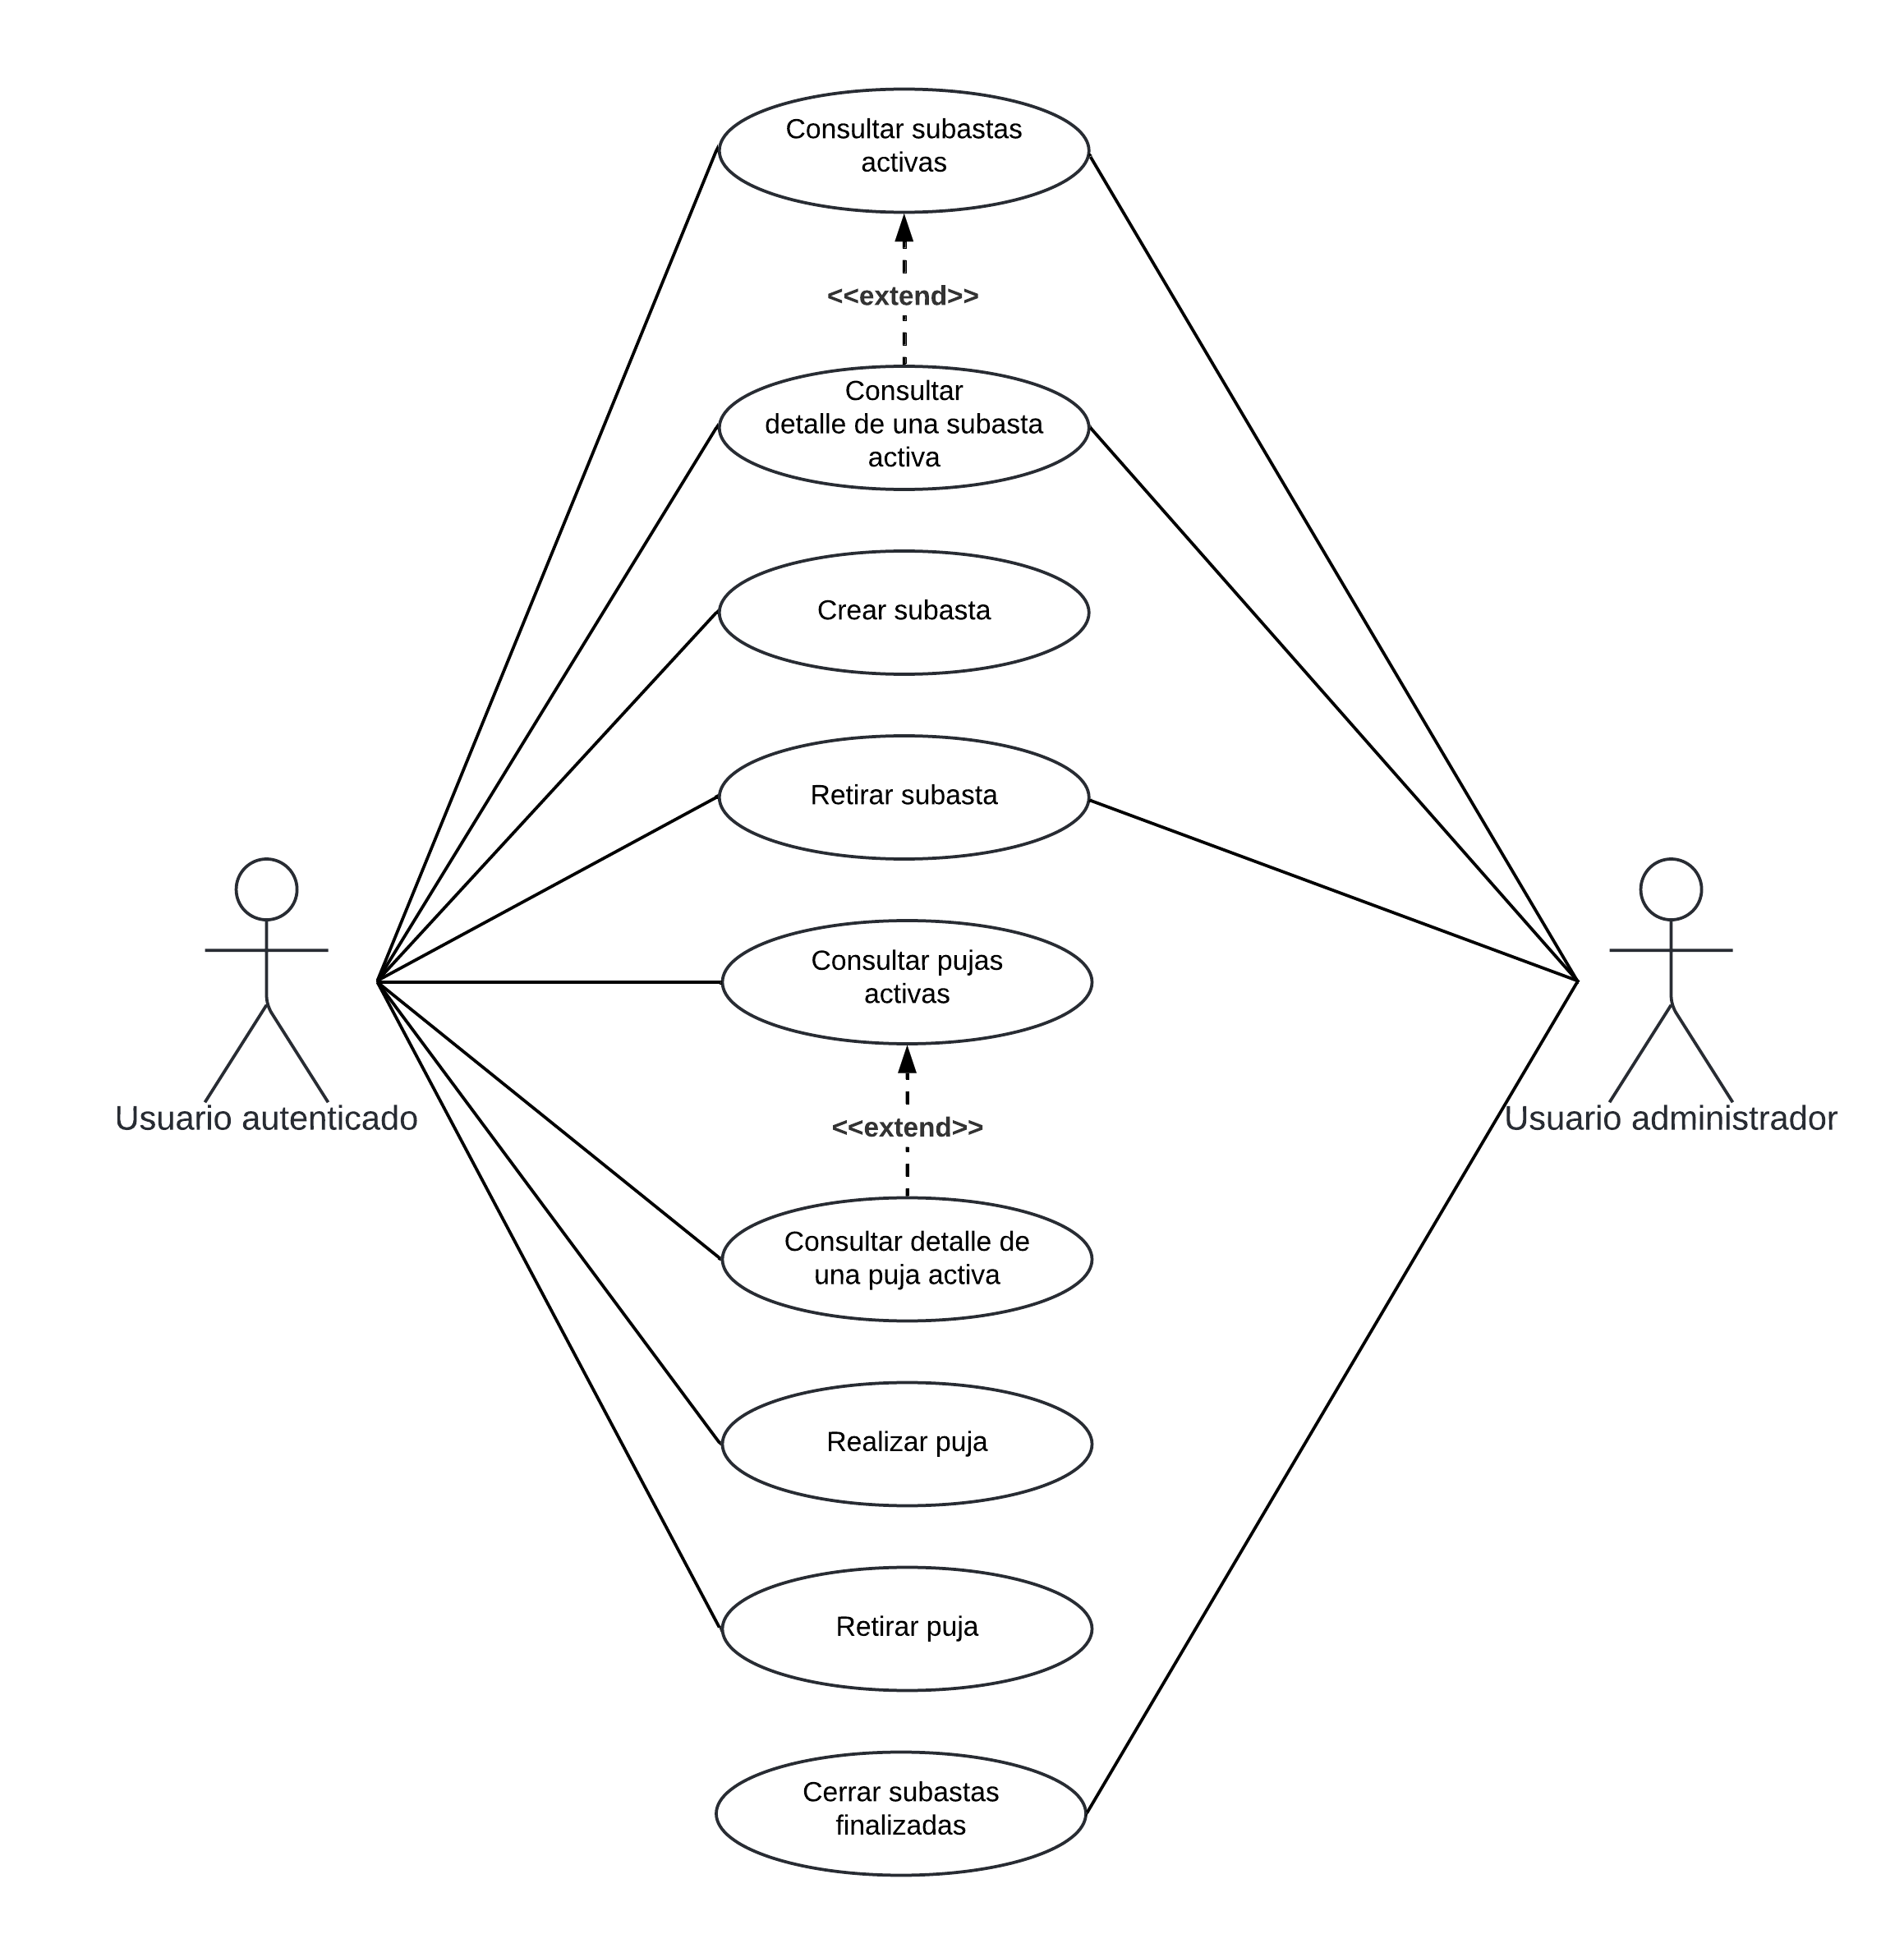
\includegraphics[width=0.5\textwidth]{figures/6-Analisis/6-Casos-uso/6_3_4_Gestion-subastas-pujas.png}
    \caption{Casos de uso. Gestión de subastas y pujas}
    \label{fig:cu_gestion-subastas-pujas}
\end{figure}

\subsubsection{Caso de uso. Crear una subasta} \label{sec:cu_crear-subasta}
\begin{longtable}{
    >{\columncolor{lightgreen!20}}p{4cm}
    p{12cm}
    }
    \caption{Caso de uso. Crear una subasta} \label{table:cu_crear-subasta} \\
    \toprule
    \rowcolor{darkgreen!50}
    \textbf{Caso de uso} & \multicolumn{1}{>{\columncolor{darkgreen!50}\centering\arraybackslash}p{12cm}}{\textbf{CREAR UNA SUBASTA}} \\
    \endfirsthead
    
    \multicolumn{2}{c}%
    {{ \tablename\ \thetable{} Caso de uso. Crear una subasta -- continuación de la página anterior}} \\
    \toprule
    \rowcolor{darkgreen!50}
    \textbf{Caso de uso} & \multicolumn{1}{>{\columncolor{darkgreen!50}\centering\arraybackslash}p{12cm}}{\textbf{CREAR UNA SUBASTA}} \\
    \midrule
    \endhead
    
    \midrule
    \multicolumn{2}{r}{{Continúa en la siguiente página...}} \\ 
    \endfoot
    
    \bottomrule
    \endlastfoot
    
    \midrule
    Descripción & Un usuario autenticado puede crear una subasta de una carta de su colección. \\
    \midrule
    Actores principales & Usuario autenticado \\
    \midrule
    Actores secundarios &  \\
    \midrule
    Precondiciones & \begin{itemize}[nosep,leftmargin=*]
        \item El usuario debe haber iniciado sesión en el sistema.
        \item El usuario debe tener al menos una carta en su colección.
        \item El usuario no debe tener ya una subasta activa para la carta que desea subastar.
    \end{itemize} \\
    \midrule
    Postcondiciones & \begin{itemize}[nosep,leftmargin=*]
        \item Se crea una nueva subasta en la base de datos.
        \item Se marca la carta como 'en subasta' en la base de datos.
    \end{itemize} \\
    \midrule
    Disparadores & El usuario accede a la sección de subastas y hace clic en el botón de crear subasta. \\
    \midrule
    Escenario principal & \begin{enumerate}[nosep,leftmargin=*]
        \item El sistema muestra el formulario de creación de subasta.
        \item El usuario selecciona la carta que desea subastar.
        \item El usuario introduce el precio de salida y la duración de la subasta.
        \item El usuario hace clic en el botón de crear subasta.
        \item El sistema valida los campos del formulario.
        \item El sistema crea una nueva subasta en la base de datos.
        \item El sistema marca la carta como 'en subasta' en la base de datos.
        \item El sistema muestra un mensaje de éxito.
        \item El sistema redirige al usuario a la página de subastas.
        \item El sistema muestra la subasta creada en la lista de subastas.
    \end{enumerate} \\
    \midrule
    Escenarios alternativos & 
    \begin{itemize}[nosep,leftmargin=*]
        \item \textbf{Escenario alternativo 1. El usuario ya tiene una subasta activa para la carta que desea subastar.}
        \begin{enumerate}[nosep,leftmargin=*]
            \item El usuario intenta crear una subasta para una carta que ya está en subasta.
            \item El sistema muestra un mensaje de error.
            \item El sistema redirige al usuario a la página de subastas.
        \end{enumerate}
        \item \textbf{Escenario alternativo 2. El usuario introduce datos inválidos.}
        \begin{enumerate}[nosep,leftmargin=*]
            \item El sistema muestra un mensaje de error.
            \item El sistema no crea la subasta en la base de datos.
            \item El sistema no marcará la carta como 'en subasta' en la base de datos.
            \item El sistema le mostrará al usuario los campos con errores.
            \item El sistema permitirá al usuario corregir los errores.
        \end{enumerate}
    \end{itemize} \\
    \midrule
    Situaciones de error & 
    \begin{itemize}[nosep,leftmargin=*]
        \item \textbf{Error de conexión a la base de datos.}
        \begin{enumerate}[nosep,leftmargin=*]
            \item El sistema mostrará un mensaje de error.
            \item El sistema no creará la subasta en la base de datos.
            \item El sistema no marcará la carta como 'en subasta' en la base de datos.
            \item El sistema redirigirá al usuario a la página de subastas.
        \end{enumerate}
    \end{itemize} \\
\end{longtable}




\subsubsection{Caso de uso. Retirar una subasta} \label{sec:cu_retirar-subasta}
\begin{longtable}{
    >{\columncolor{lightgreen!20}}p{4cm}
    p{12cm}
    }
    \caption{Caso de uso. Retirar una subasta} \label{table:cu_retirar-subasta} \\
    \toprule
    \rowcolor{darkgreen!50}
    \textbf{Caso de uso} & \multicolumn{1}{>{\columncolor{darkgreen!50}\centering\arraybackslash}p{12cm}}{\textbf{RETIRAR UNA SUBASTA}} \\
    \endfirsthead
    
    \multicolumn{2}{c}%
    {{ \tablename\ \thetable{} Caso de uso. Retirar una subasta -- continuación de la página anterior}} \\
    \toprule
    \rowcolor{darkgreen!50}
    \textbf{Caso de uso} & \multicolumn{1}{>{\columncolor{darkgreen!50}\centering\arraybackslash}p{12cm}}{\textbf{RETIRAR UNA SUBASTA}} \\
    \midrule
    \endhead
    
    \midrule
    \multicolumn{2}{r}{{Continúa en la siguiente página...}} \\ 
    \endfoot
    
    \bottomrule
    \endlastfoot
    
    \midrule
    Descripción & Un usuario autenticado puede retirar una subasta activa en el sistema si es el vendedor de la subasta. Un usuario administrador puede retirar cualquier subasta activa en el sistema. \\
    \midrule
    Actores principales & Usuario autenticado o usuario administrador \\
    \midrule
    Actores secundarios &  \\
    \midrule
    Precondiciones & \begin{itemize}[nosep,leftmargin=*]
        \item El usuario debe haber iniciado sesión en el sistema.
        \item El usuario debe tener al menos una subasta activa.
    \end{itemize} \\
    \midrule
    Postcondiciones & \begin{itemize}[nosep,leftmargin=*]
        \item Se marca la subasta como 'cancelada' en la base de datos.
        \item La carta subastada vuelve a estar disponible en la colección del usuario.
        \item Se actualizan las pujas de la subasta en la base de datos, marcando las pujas como 'canceladas'.
        \item Se informa a los usuarios que hayan pujado en la subasta de que ha sido cancelada.
        \item Si la subasta ha sido retirada por un administrador, se notifica al usuario vendedor de la subasta en tiempo real.
    \end{itemize} \\
    \midrule
    Disparadores & El usuario accede a la sección de subastas y hace clic en el botón de retirar subasta. \\
    \midrule
    Escenario principal & \begin{enumerate}[nosep,leftmargin=*]
        \item El sistema muestra la lista de subastas activas del usuario.
        \item El usuario selecciona la subasta que desea retirar.
        \item El usuario hace clic en el botón de retirar subasta.
        \item El sistema muestra un mensaje de confirmación.
        \item El usuario confirma la retirada de la subasta.
        \item El sistema marca la subasta como 'cancelada' en la base de datos.
        \item La carta subastada vuelve a estar disponible en la colección del usuario.
        \item El sistema muestra un mensaje de éxito.
        \item El sistema redirige al usuario a la página de subastas.
    \end{enumerate} \\
    \midrule
    Escenarios alternativos & 
    \begin{itemize}[nosep,leftmargin=*]
        \item \textbf{Escenario alternativo 1. El usuario cancela la retirada de la subasta.}
        \begin{enumerate}[nosep,leftmargin=*]
            \item El usuario hace clic en el botón de cancelar en el mensaje de confirmación.
            \item El sistema no marcará la subasta como 'cancelada' en la base de datos.
            \item El sistema redirigirá al usuario a la página de subastas.
        \end{enumerate}
    \end{itemize} \\
    \midrule
    Situaciones de error & 
    \begin{itemize}[nosep,leftmargin=*]
        \item \textbf{Error de conexión a la base de datos.}
        \begin{enumerate}[nosep,leftmargin=*]
            \item El sistema mostrará un mensaje de error.
            \item El sistema no marcará la subasta como 'cancelada' en la base de datos.
            \item El sistema no devolverá la carta subastada a la colección del usuario.
            \item El sistema redirigirá al usuario a la página de subastas.
        \end{enumerate}
    \end{itemize} \\
\end{longtable}




\subsubsection{Caso de uso. Consultar subastas activas} \label{sec:cu_consultar-subastas}
\begin{longtable}{
    >{\columncolor{lightgreen!20}}p{4cm}
    p{12cm}
    }
    \caption{Caso de uso. Consultar subastas activas} \label{table:cu_consultar-subastas} \\
    \toprule
    \rowcolor{darkgreen!50}
    \textbf{Caso de uso} & \multicolumn{1}{>{\columncolor{darkgreen!50}\centering\arraybackslash}p{12cm}}{\textbf{CONSULTAR SUBASTAS ACTIVAS}} \\
    \endfirsthead
    
    \multicolumn{2}{c}%
    {{ \tablename\ \thetable{} Caso de uso. Consultar subastas activas -- continuación de la página anterior}} \\
    \toprule
    \rowcolor{darkgreen!50}
    \textbf{Caso de uso} & \multicolumn{1}{>{\columncolor{darkgreen!50}\centering\arraybackslash}p{12cm}}{\textbf{CONSULTAR SUBASTAS ACTIVAS}} \\
    \midrule
    \endhead
    
    \midrule
    \multicolumn{2}{r}{{Continúa en la siguiente página...}} \\ 
    \endfoot
    
    \bottomrule
    \endlastfoot
    
    \midrule
    Descripción & Un usuario autenticado o administrador puede consultar las subastas activas en el sistema. \\
    \midrule
    Actores principales & Usuario autenticado o usuario administrador \\
    \midrule
    Actores secundarios &  \\
    \midrule
    Precondiciones & \begin{itemize}[nosep,leftmargin=*]
        \item El usuario debe haber iniciado sesión en el sistema.
    \end{itemize} \\
    \midrule
    Postcondiciones &  \\
    \midrule
    Disparadores & El usuario accede a la sección de subastas. \\
    \midrule
    Escenario principal & \begin{enumerate}[nosep,leftmargin=*]
        \item El sistema muestra la lista de subastas activas.
        \item El usuario puede seleccionar una subasta para ver su información detallada.
    \end{enumerate} \\
    \midrule
    Escenarios alternativos & 
    \begin{itemize}[nosep,leftmargin=*]
        \item \textbf{Escenario alternativo 1. No hay subastas activas.}
        \begin{enumerate}[nosep,leftmargin=*]
            \item El sistema mostrará un mensaje indicando que no hay subastas activas.
        \end{enumerate}
        \item \textbf{Escenario alternativo 2. El usuario consulta sus propias subastas.} 
        \begin{enumerate}[nosep,leftmargin=*]
            \item El usuario accede a la sección de subastas.
            \item El sistema muestra la opción de ver las subastas activas del usuario.
            \item El usuario selecciona la opción de ver sus propias subastas.
            \item El sistema muestra la lista de subastas activas del usuario.
            \item El usuario puede seleccionar una subasta para ver su información detallada.
        \end{enumerate}
        \item \textbf{Escenario alternativo 3. Un usuario administrador consulta las subastas activas.}
        \begin{enumerate}[nosep,leftmargin=*]
            \item El usuario administrador accede a la sección de subastas.
            \item El sistema muestra la lista de subastas activas de todos los usuarios.
            \item El usuario administrador puede seleccionar una subasta para ver su información detallada.
        \end{enumerate}
    \end{itemize} \\
    \midrule
    Situaciones de error & 
    \begin{itemize}[nosep,leftmargin=*]
        \item \textbf{Error de conexión a la base de datos.}
        \begin{enumerate}[nosep,leftmargin=*]
            \item El sistema mostrará un mensaje de error.
        \end{enumerate}
    \end{itemize} \\
\end{longtable}

\subsubsection{Caso de uso. Consultar el detalle de una subasta activa} \label{sec:cu_consultar-detalle-subasta}
\begin{longtable}{
    >{\columncolor{lightgreen!20}}p{4cm}
    p{12cm}
    }
    \caption{Caso de uso. Consultar el detalle de una subasta activa} \label{table:cu_consultar-detalle-subasta} \\
    \toprule
    \rowcolor{darkgreen!50}
    \textbf{Caso de uso} & \multicolumn{1}{>{\columncolor{darkgreen!50}\centering\arraybackslash}p{12cm}}{\textbf{CONSULTAR DETALLE DE UNA SUBASTA ACTIVA}} \\
    \endfirsthead
    
    \multicolumn{2}{c}%
    {{ \tablename\ \thetable{} Caso de uso. Consultar el detalle de una subasta activa -- continuación de la página anterior}} \\
    \toprule
    \rowcolor{darkgreen!50}
    \textbf{Caso de uso} & \multicolumn{1}{>{\columncolor{darkgreen!50}\centering\arraybackslash}p{12cm}}{\textbf{CONSULTAR DETALLE DE UNA SUBASTA ACTIVA}} \\
    \midrule
    \endhead
    
    \midrule
    \multicolumn{2}{r}{{Continúa en la siguiente página...}} \\ 
    \endfoot
    
    \bottomrule
    \endlastfoot
    
    \midrule
    Descripción & Un usuario autenticado o administrador puede consultar el detalle de una subasta activa en el sistema. \\
    \midrule
    Actores principales & Usuario autenticado o usuario administrador \\
    \midrule
    Actores secundarios &  \\
    \midrule
    Precondiciones & \begin{itemize}[nosep,leftmargin=*]
        \item El usuario debe haber iniciado sesión en el sistema.
    \end{itemize} \\
    \midrule
    Postcondiciones &  \\
    \midrule
    Disparadores & El usuario accede a la sección de subastas y selecciona una subasta activa. \\
    \midrule
    Escenario principal & \begin{enumerate}[nosep,leftmargin=*]
        \item El usuario selecciona una subasta activa.
        \item El sistema muestra la información detallada de la carta subastada, incluido el histórico de transacciones de esta.
        \item El sistema muestra la duración restante de la subasta.
    \end{enumerate} \\
    \midrule
    Escenarios alternativos & 
    \begin{itemize}[nosep,leftmargin=*]
        \item \textbf{Escenario alternativo 1. El usuario que consulta la subasta es el propietario de la subasta.}
        \begin{enumerate}[nosep,leftmargin=*]
            \item El usuario selecciona una subasta activa.
            \item El sistema muestra la información detallada de la carta subastada, incluido el histórico de transacciones de esta.
            \item El sistema muestra la duración restante de la subasta.
            \item El sistema muestra el precio de salida establecido por el usuario.
            \item El sistema muestra la opción de retirar la subasta.
        \end{enumerate}
        \item \textbf{Escenario alternativo 3. Un usuario administrador consulta la subasta.}
        \begin{enumerate}[nosep,leftmargin=*]
            \item El usuario administrador selecciona una subasta activa.
            \item El sistema muestra la información detallada de la carta subastada, incluido el histórico de transacciones de esta.
            \item El sistema muestra la duración restante de la subasta.
            \item El sistema muestra el precio de salida establecido por el vendedor.
            \item El sistema muestra la opción de retirar la subasta.
        \end{enumerate}
    \end{itemize} \\
    \midrule
    Situaciones de error & 
    \begin{itemize}[nosep,leftmargin=*]
        \item \textbf{Error de conexión a la base de datos.}
        \begin{enumerate}[nosep,leftmargin=*]
            \item El sistema mostrará un mensaje de error.
        \end{enumerate}
    \end{itemize} \\
\end{longtable}


\subsubsection{Caso de uso. Realizar puja} \label{sec:cu_realizar-puja}
\begin{longtable}{
    >{\columncolor{lightgreen!20}}p{4cm}
    p{12cm}
    }
    \caption{Caso de uso. Realizar puja} \label{table:cu_realizar-puja} \\
    \toprule
    \rowcolor{darkgreen!50}
    \textbf{Caso de uso} & \multicolumn{1}{>{\columncolor{darkgreen!50}\centering\arraybackslash}p{12cm}}{\textbf{REALIZAR PUJA}} \\
    \endfirsthead
    
    \multicolumn{2}{c}%
    {{ \tablename\ \thetable{} Caso de uso. Realizar puja -- continuación de la página anterior}} \\
    \toprule
    \rowcolor{darkgreen!50}
    \textbf{Caso de uso} & \multicolumn{1}{>{\columncolor{darkgreen!50}\centering\arraybackslash}p{12cm}}{\textbf{REALIZAR PUJA}} \\
    \midrule
    \endhead
    
    \midrule
    \multicolumn{2}{r}{{Continúa en la siguiente página...}} \\ 
    \endfoot
    
    \bottomrule
    \endlastfoot
    
    \midrule
    Descripción & Un usuario autenticado puede realizar una puja en una subasta activa. \\
    \midrule
    Actores principales & Usuario autenticado \\
    \midrule
    Actores secundarios &  \\
    \midrule
    Precondiciones & \begin{itemize}[nosep,leftmargin=*]
        \item El usuario debe haber iniciado sesión en el sistema.
        \item El usuario debe tener saldo suficiente para realizar la puja.
    \end{itemize} \\
    \midrule
    Postcondiciones & \begin{itemize}[nosep,leftmargin=*]
        \item Se registra la puja en la base de datos.
    \end{itemize} \\
    \midrule
    Disparadores & El usuario selecciona una subasta activa y hace clic en el botón de realizar puja. \\
    \midrule
    Escenario principal & \begin{enumerate}[nosep,leftmargin=*]
        \item El sistema muestra la información detallada de la subasta.
        \item El usuario introduce la cantidad de la puja.
        \item El usuario hace clic en el botón de realizar puja.
        \item El sistema valida la cantidad de la puja.
        \item El sistema registra la puja en la base de datos.
        \item El sistema muestra un mensaje de éxito.
        \item El sistema muestra un mensaje informativo, indicando que si en el momento de finalización del tiempo de la subasta no cuenta con el saldo suficiente, la puja no será válida.
        \item El sistema redirige al usuario a la página de subastas.
    \end{enumerate} \\
    \midrule
    Escenarios alternativos & 
    \begin{itemize}[nosep,leftmargin=*]
        \item \textbf{Escenario alternativo 1. El usuario no tiene saldo suficiente para realizar la puja.}
        \begin{enumerate}[nosep,leftmargin=*]
            \item El usuario intenta realizar una puja sin tener saldo suficiente.
            \item El sistema mostrará un mensaje de error.
            \item El sistema no registrará la puja en la base de datos.
            \item El sistema redirigirá al usuario a la página de subastas.
        \end{enumerate}
        \item \textbf{Escenario alternativo 2. El usuario introduce una cantidad de puja inválida.}
        \begin{enumerate}[nosep,leftmargin=*]
            \item El sistema mostrará un mensaje de error.
            \item El sistema no registrará la puja en la base de datos.
            \item El sistema le mostrará al usuario los campos con errores.
            \item El sistema permitirá al usuario corregir los errores.
        \end{enumerate}
    \end{itemize} \\
    \midrule
    Situaciones de error & 
    \begin{itemize}[nosep,leftmargin=*]
        \item \textbf{Error de conexión a la base de datos.}
        \begin{enumerate}[nosep,leftmargin=*]
            \item El sistema mostrará un mensaje de error.
            \item El sistema no registrará la puja en la base de datos.
            \item El sistema redirigirá al usuario a la página de subastas.
        \end{enumerate}
    \end{itemize} \\
\end{longtable}



\subsubsection{Caso de uso. Retirar puja} \label{sec:cu_retirar-puja}
\begin{longtable}{
    >{\columncolor{lightgreen!20}}p{4cm}
    p{12cm}
    }
    \caption{Caso de uso. Retirar puja} \label{table:cu_retirar-puja} \\
    \toprule
    \rowcolor{darkgreen!50}
    \textbf{Caso de uso} & \multicolumn{1}{>{\columncolor{darkgreen!50}\centering\arraybackslash}p{12cm}}{\textbf{RETIRAR PUJA}} \\
    \endfirsthead
    
    \multicolumn{2}{c}%
    {{ \tablename\ \thetable{} Caso de uso. Retirar puja -- continuación de la página anterior}} \\
    \toprule
    \rowcolor{darkgreen!50}
    \textbf{Caso de uso} & \multicolumn{1}{>{\columncolor{darkgreen!50}\centering\arraybackslash}p{12cm}}{\textbf{RETIRAR PUJA}} \\
    \midrule
    \endhead
    
    \midrule
    \multicolumn{2}{r}{{Continúa en la siguiente página...}} \\ 
    \endfoot
    
    \bottomrule
    \endlastfoot
    
    \midrule
    Descripción & Un usuario podrá retirar una puja realizada en una subasta activa. \\
    \midrule
    Actores principales & Usuario autenticado \\
    \midrule
    Actores secundarios &  \\
    \midrule
    Precondiciones & \begin{itemize}[nosep,leftmargin=*]
        \item El usuario debe haber iniciado sesión en el sistema.
        \item El usuario debe haber realizado una puja en una subasta activa.
        \item La subasta no debe haber finalizado.
    \end{itemize} \\
    \midrule
    Postcondiciones & \begin{itemize}[nosep,leftmargin=*]
        \item Se actualiza la puja en la base de datos, marcándola como 'retirada'.
        \item La puja no se muestra en la lista de pujas activas del usuario.
        \item La puja no se tendr´a en cuenta en el cálculo de la puja más alta.
    \end{itemize} \\
    \midrule
    Disparadores & El usuario accede a la sección de pujas activas, selecciona una puja y hace clic en el botón de retirar puja. \\
    \midrule
    Escenario principal & \begin{enumerate}[nosep,leftmargin=*]
        \item El sistema muestra la lista de pujas activas del usuario.
        \item El usuario selecciona la puja que desea retirar.
        \item El usuario hace clic en el botón de retirar puja.
        \item El sistema muestra un mensaje de confirmación.
        \item El usuario confirma la retirada de la puja.
        \item El sistema actualiza la puja en la base de datos, marcándola como 'retirada'.
        \item El sistema muestra un mensaje de éxito.
        \item El sistema redirige al usuario a la página de subastas.
    \end{enumerate} \\
    \midrule
    Escenarios alternativos & 
    \begin{itemize}[nosep,leftmargin=*]
        \item \textbf{Escenario alternativo 1. El usuario cancela la retirada de la puja.}
        \begin{enumerate}[nosep,leftmargin=*]
            \item El usuario hace clic en el botón de cancelar en el mensaje de confirmación.
            \item El sistema no marcará la puja como 'retirada' en la base de datos.
            \item El sistema redirigirá al usuario a la página de subastas.
        \end{enumerate}
    \end{itemize} \\
    \midrule
    Situaciones de error & 
    \begin{itemize}[nosep,leftmargin=*]
        \item \textbf{Error de conexión a la base de datos.}
        \begin{enumerate}[nosep,leftmargin=*]
            \item El sistema mostrará un mensaje de error.
            \item El sistema redirigirá al usuario a la página de subastas.
        \end{enumerate}
    \end{itemize} \\
\end{longtable}




\subsubsection{Caso de uso. Consultar pujas activas} \label{sec:cu_consultar-pujas}
\begin{longtable}{
    >{\columncolor{lightgreen!20}}p{4cm}
    p{12cm}
    }
    \caption{Caso de uso. Consultar pujas activas} \label{table:cu_consultar-pujas} \\
    \toprule
    \rowcolor{darkgreen!50}
    \textbf{Caso de uso} & \multicolumn{1}{>{\columncolor{darkgreen!50}\centering\arraybackslash}p{12cm}}{\textbf{CONSULTAR PUJAS ACTIVAS}} \\
    \endfirsthead
    
    \multicolumn{2}{c}%
    {{ \tablename\ \thetable{} Caso de uso. Consultar pujas activas -- continuación de la página anterior}} \\
    \toprule
    \rowcolor{darkgreen!50}
    \textbf{Caso de uso} & \multicolumn{1}{>{\columncolor{darkgreen!50}\centering\arraybackslash}p{12cm}}{\textbf{CONSULTAR PUJAS ACTIVAS}} \\
    \midrule
    \endhead
    
    \midrule
    \multicolumn{2}{r}{{Continúa en la siguiente página...}} \\ 
    \endfoot
    
    \bottomrule
    \endlastfoot
    
    \midrule
    Descripción & Un usuario autenticado puede consultar las pujas activas en las subastas en las que ha participado. \\
    \midrule
    Actores principales & Usuario autenticado o usuario administrador \\
    \midrule
    Actores secundarios &  \\
    \midrule
    Precondiciones & \begin{itemize}[nosep,leftmargin=*]
        \item El usuario debe haber iniciado sesión en el sistema.
    \end{itemize} \\
    \midrule
    Postcondiciones &  \\
    \midrule
    Disparadores & El usuario accede a la sección de subastas y hace clic en el botón de consultar pujas activas. \\
    \midrule
    Escenario principal & \begin{enumerate}[nosep,leftmargin=*]
        \item El sistema muestra la lista de pujas activas.
        \item El usuario puede seleccionar una puja para ver su información detallada.
    \end{enumerate} \\
    \midrule
    Escenarios alternativos & 
    \begin{itemize}[nosep,leftmargin=*]
        \item \textbf{Escenario alternativo 1. No hay pujas activas.}
        \begin{enumerate}[nosep,leftmargin=*]
            \item El sistema mostrará un mensaje indicando que no hay pujas activas.
        \end{enumerate}
    \end{itemize} \\
    \midrule
    Situaciones de error & 
    \begin{itemize}[nosep,leftmargin=*]
        \item \textbf{Error de conexión a la base de datos.}
        \begin{enumerate}[nosep,leftmargin=*]
            \item El sistema mostrará un mensaje de error.
        \end{enumerate}
    \end{itemize} \\
\end{longtable}

\subsubsection{Caso de uso. Consultar el detalle de una puja activa} \label{sec:cu_consultar-detalle-puja}
\begin{longtable}{
    >{\columncolor{lightgreen!20}}p{4cm}
    p{12cm}
    }
    \caption{Caso de uso. Consultar el detalle de una puja activa} \label{table:cu_consultar-detalle-puja} \\
    \toprule
    \rowcolor{darkgreen!50}
    \textbf{Caso de uso} & \multicolumn{1}{>{\columncolor{darkgreen!50}\centering\arraybackslash}p{12cm}}{\textbf{CONSULTAR DETALLE DE UNA PUJA ACTIVA}} \\
    \endfirsthead
    
    \multicolumn{2}{c}%
    {{ \tablename\ \thetable{} Caso de uso. Consultar el detalle de una puja activa -- continuación de la página anterior}} \\
    \toprule
    \rowcolor{darkgreen!50}
    \textbf{Caso de uso} & \multicolumn{1}{>{\columncolor{darkgreen!50}\centering\arraybackslash}p{12cm}}{\textbf{CONSULTAR DETALLE DE UNA PUJA ACTIVA}} \\
    \midrule
    \endhead
    
    \midrule
    \multicolumn{2}{r}{{Continúa en la siguiente página...}} \\ 
    \endfoot
    
    \bottomrule
    \endlastfoot
    
    \midrule
    Descripción & Un usuario autenticado puede consultar el detalle de una puja activa en el sistema. \\
    \midrule
    Actores principales & Usuario autenticado \\
    \midrule
    Actores secundarios &  \\
    \midrule
    Precondiciones & \begin{itemize}[nosep,leftmargin=*]
        \item El usuario debe haber iniciado sesión en el sistema.
    \end{itemize} \\
    \midrule
    Postcondiciones &  \\
    \midrule
    Disparadores & El usuario accede a la sección de pujas activas y selecciona una puja activa. \\
    \midrule
    Escenario principal & \begin{enumerate}[nosep,leftmargin=*]
        \item El usuario selecciona una puja activa.
        \item El sistema muestra la información detallada de la carta subastada, incluido el histórico de transacciones de esta.
        \item El sistema muestra la duración restante de la subasta.
        \item El sistema muestra la cantidad de la puja.
        \item El sistema muestra la opción de retirar la puja.
    \end{enumerate} \\
    \midrule
    Escenarios alternativos &  \\
    \midrule
    Situaciones de error & 
    \begin{itemize}[nosep,leftmargin=*]
        \item \textbf{Error de conexión a la base de datos.}
        \begin{enumerate}[nosep,leftmargin=*]
            \item El sistema mostrará un mensaje de error.
        \end{enumerate}
    \end{itemize} \\
\end{longtable}


\subsubsection{Caso de uso. Cerrar subastas finalizadas} \label{sec:cu_cerrar-subastas}
\begin{longtable}{
    >{\columncolor{lightgreen!20}}p{4cm}
    p{12cm}
    }
    \caption{Caso de uso. Cerrar subastas finalizadas} \label{table:cu_cerrar-subastas} \\
    \toprule
    \rowcolor{darkgreen!50}
    \textbf{Caso de uso} & \multicolumn{1}{>{\columncolor{darkgreen!50}\centering\arraybackslash}p{12cm}}{\textbf{CERRAR SUBASTAS FINALIZADAS}} \\
    \endfirsthead
    
    \multicolumn{2}{c}%
    {{ \tablename\ \thetable{} Caso de uso. Cerrar subastas finalizadas -- continuación de la página anterior}} \\
    \toprule
    \rowcolor{darkgreen!50}
    \textbf{Caso de uso} & \multicolumn{1}{>{\columncolor{darkgreen!50}\centering\arraybackslash}p{12cm}}{\textbf{CERRAR SUBASTAS FINALIZADAS}} \\
    \midrule
    \endhead
    
    \midrule
    \multicolumn{2}{r}{{Continúa en la siguiente página...}} \\ 
    \endfoot
    
    \bottomrule
    \endlastfoot
    
    \midrule
    Descripción & Un usuario administrador podrá cerrar las subastas que hayan finalizado. El sistema se encargará de procesar las pujas, notificar a los usuarios ganadores y transferir la carta. \\
    \midrule
    Actores principales & Usuario administrador \\
    \midrule
    Actores secundarios &  \\
    \midrule
    Precondiciones & \begin{itemize}[nosep,leftmargin=*]
        \item El usuario debe haber iniciado sesión en el sistema.
    \end{itemize} \\
    \midrule
    Postcondiciones & 
    \begin{itemize}[nosep,leftmargin=*]
        \item Se marcan las subastas como 'cerradas' en la base de datos.
        \item Se actualiza la información de las cartas subastadas en la base de datos.
        \item Se notifica a los dueños de las cartas subastadas del resultado de la subasta.
        \item Se notifica a los usuarios ganadores de las subastas si los hubiera.
        \item Se transfiere el monto de la puja ganadora a la cuenta del vendedor.
        \item Se descuenta el monto de la puja ganadora de la cuenta del usuario ganador.
        \item Se transfiere la carta subastada a los usuarios ganadores.
        \item Se registran las transacciones en la base de datos.
    \end{itemize} \\
    \midrule
    Disparadores & El usuario accede a la sección de subastas activas y hace clic en el botón de cerrar subastas. \\
    \midrule
    Escenario principal & \begin{enumerate}[nosep,leftmargin=*]
        \item El usuario selecciona la opción de cerrar subastas.
        \item El sistema muestra la lista de subastas finalizadas que han sido cerradas con sus resultados.
        \item El sistema informa a los dueños de las cartas subastadas del resultado de la subasta.
        \item El sistema informa a los usuarios ganadores de las subastas si los hubiera.
    \end{enumerate} \\
    \midrule
    Escenarios alternativos &  
    \begin{itemize}[nosep,leftmargin=*]
        \item \textbf{Escenario alternativo 1. No hay subastas finalizadas.}
        \begin{enumerate}[nosep,leftmargin=*]
            \item El sistema mostrará un mensaje indicando que no hay subastas que cerrar.
        \end{enumerate}
    \end{itemize} \\
    \midrule
    Situaciones de error & 
    \begin{itemize}[nosep,leftmargin=*]
        \item \textbf{Error de conexión a la base de datos.}
        \begin{enumerate}[nosep,leftmargin=*]
            \item El sistema mostrará un mensaje de error.
        \end{enumerate}
    \end{itemize} \\
\end{longtable}

\subsubsubsection{Diagrama de secuencia. Cerrar subastas finalizadas} \label{sec:dsec_cerrar-subastas}
En la figura \ref{fig:seq-cerrar-subastas} se muestra el diagrama de secuencia correspondiente al caso de uso \textit{Cerrar subastas finalizadas}.
\begin{figure}[H]
    \centering
     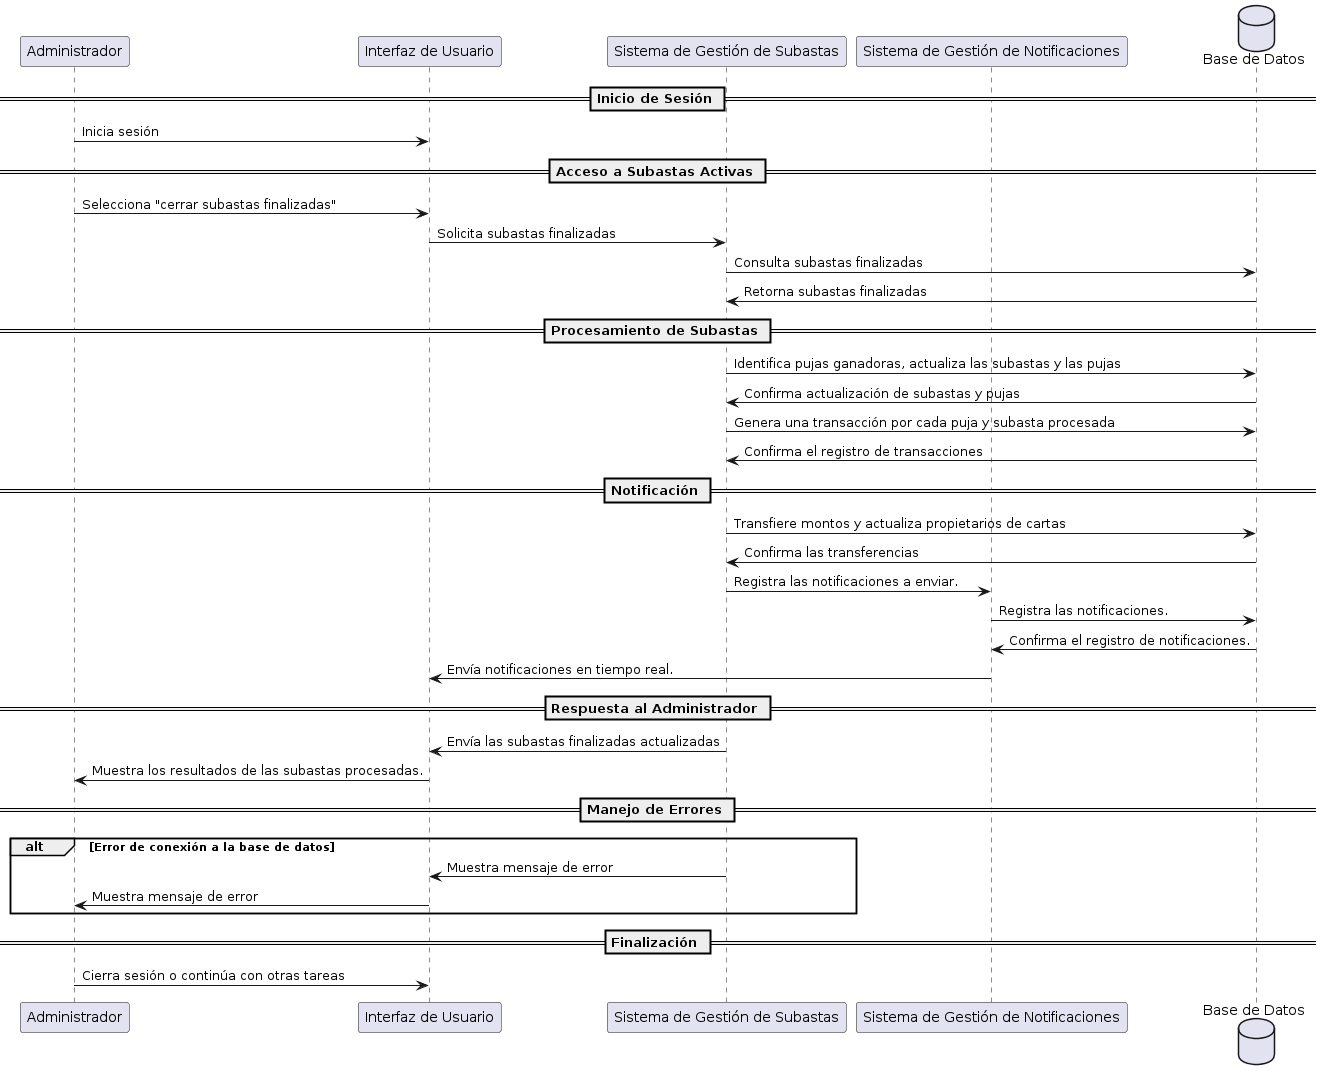
\includegraphics[width=1\textwidth]{figures/6-Analisis/6-Casos-uso/6_3_4_DSec-cerrar-subastas.png}
    \caption{Diagrama de secuencia. Cerrar subastas finalizadas}
    \label{fig:seq-cerrar-subastas}
\end{figure}

\newpage
\subsection{Casos de uso. Gestión de transacciones}
\begin{figure}[H]
    \centering
    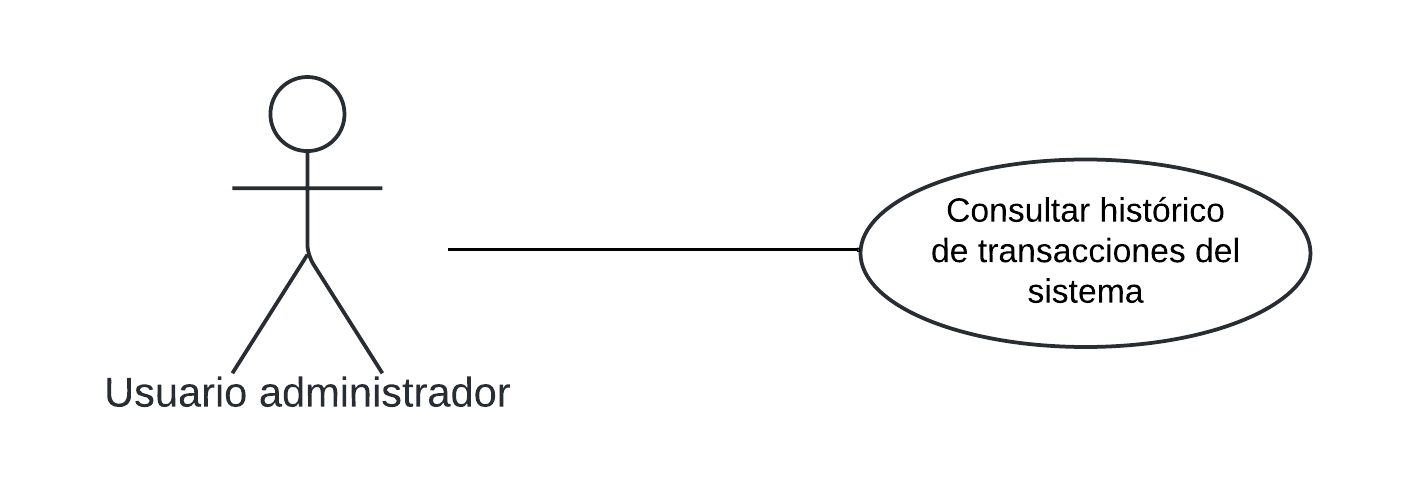
\includegraphics[width=0.5\textwidth]{figures/6-Analisis/6-Casos-uso/6_3_5_Gestion-transacciones.png}
    \caption{Casos de uso. Gestión de transacciones}
    \label{fig:cu_gestion-transacciones}
\end{figure}

\subsubsection{Caso de uso. Consultar histórico de transacciones del sistema} \label{sec:cu_transacciones-sistema}
\begin{longtable}{
   >{\columncolor{lightgreen!20}}p{4cm} % Primera columna con color de fondo verde claro
    >{\columncolor{white}}p{12cm}        % Segunda columna con color de fondo blanco (explícito)
    }
    \caption{Caso de uso. Histórico de transacciones del sistema} \label{table:cu_transacciones-sistema} \\
    \toprule
    \rowcolor{darkgreen!50} % Aplicando color de fondo verde oscuro a toda la fila
    \textbf{Caso de uso} & \centering\arraybackslash \textbf{HISTÓRICO DE TRANSACCIONES DEL SISTEMA} \\
    \endfirsthead
    
    \multicolumn{2}{c}%
    {\tablename\ \thetable{} -- continuación de la página anterior} \\
    \toprule
    \rowcolor{darkgreen!50}
    \textbf{Caso de uso} & \centering\arraybackslash \textbf{HISTÓRICO DE TRANSACCIONES DEL SISTEMA} \\
    \midrule
    \endhead
    
    \midrule
    \multicolumn{2}{r}{Continúa en la siguiente página...} \\ 
    \endfoot
    
    \bottomrule
    \endlastfoot
    
    \midrule
    Descripción & Un usuario administrador puede consultar el histórico de transacciones del sistema. \\
    \midrule
    Actores principales & Usuario administrador \\
    \midrule
    Actores secundarios &  \\
    \midrule
    Precondiciones & \begin{itemize}[nosep,leftmargin=*]
        \item El usuario ha iniciado sesión en el sistema.
    \end{itemize} \\
    \midrule
    Postcondiciones &  \\
    \midrule
    Disparadores & El usuario selecciona la opción de consultar el histórico de transacciones. \\
    \midrule
    Escenario principal & \begin{enumerate}[nosep,leftmargin=*]
        \item El sistema muestra el listado de transacciones realizadas en el sistema por los diferentes usuarios.
        \item El usuario puede filtrar las transacciones por diferentes criterios.
    \end{enumerate} \\
    \midrule
    Escenarios alternativos & 
    \begin{itemize}[nosep,leftmargin=*]
        \item \textbf{Escenario alternativo 1. No hay transacciones registradas.}
        \begin{enumerate}[nosep,leftmargin=*]
            \item El sistema muestra un mensaje indicando que no hay transacciones registradas.
        \end{enumerate}
    \end{itemize} \\
    \midrule
    Situaciones de error & 
    \begin{itemize}[nosep,leftmargin=*]
        \item \textbf{Error de conexión a la base de datos.}
        \begin{enumerate}[nosep,leftmargin=*]
            \item El sistema muestra un mensaje de error.
        \end{enumerate}
    \end{itemize} \\
\end{longtable}



\newpage
\subsection{Casos de uso. Gestión de notificaciones}
\begin{figure}[H]
    \centering
    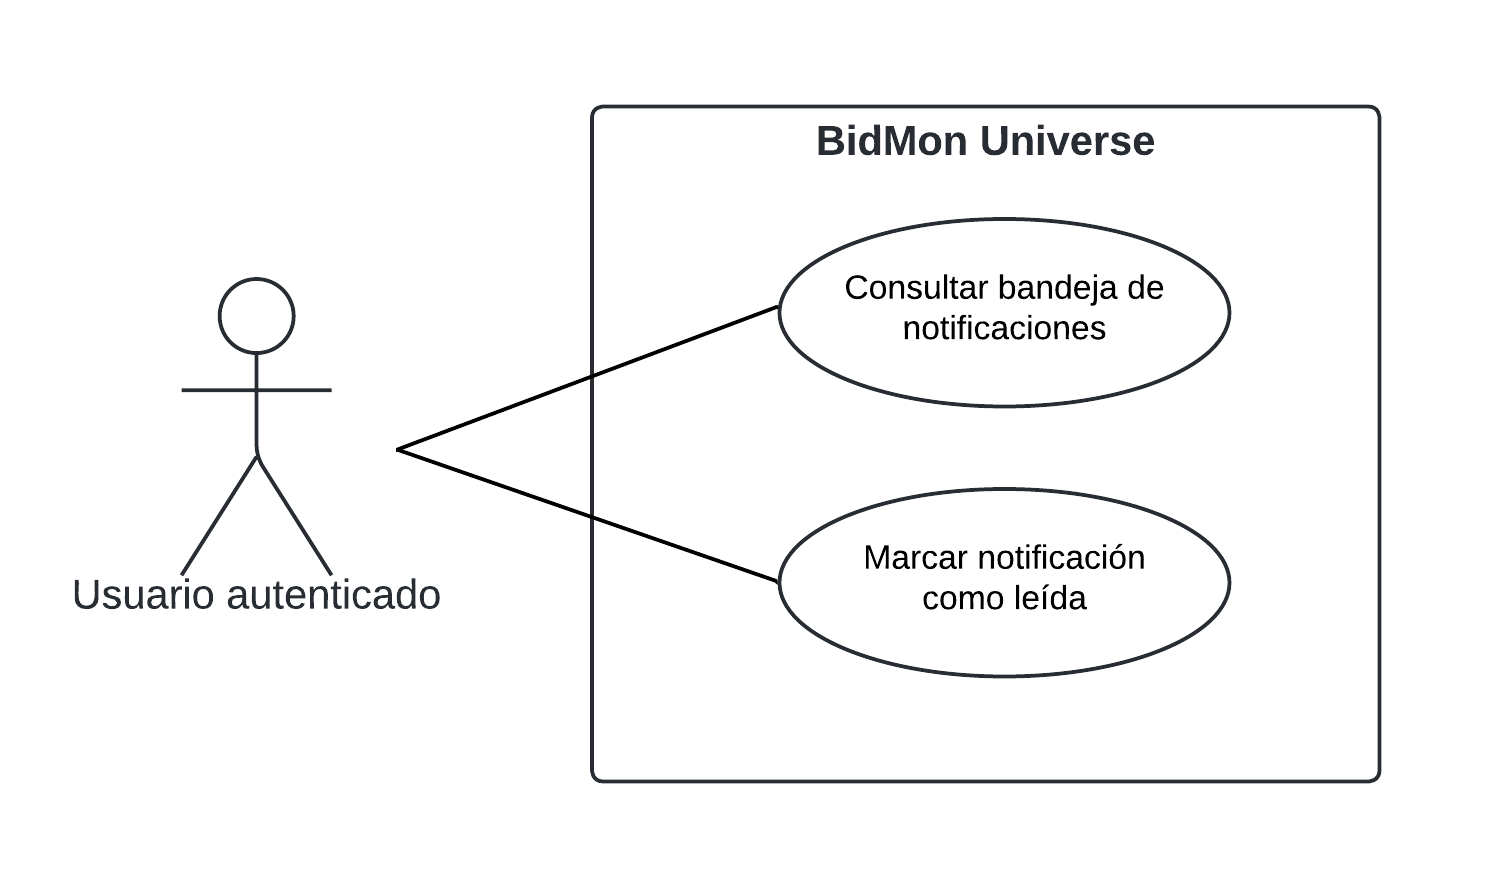
\includegraphics[width=0.5\textwidth]{figures/6-Analisis/6-Casos-uso/6_3_6_Gestion-notificaciones.png}
    \caption{Casos de uso. Gestión de notificaciones}
    \label{fig:cu_gestion-notificaciones}
\end{figure}

\subsubsection{Caso de uso. Consultar bandeja de notificaciones} \label{sec:cu_notificaciones}
\begin{longtable}{
   >{\columncolor{lightgreen!20}}p{4cm} % Primera columna con color de fondo verde claro
    >{\columncolor{white}}p{12cm}        % Segunda columna con color de fondo blanco (explícito)
    }
    \caption{Caso de uso. Consultar bandeja de notificaciones} \label{table:cu_notificaciones} \\
    \toprule
    \rowcolor{darkgreen!50} % Aplicando color de fondo verde oscuro a toda la fila
    \textbf{Caso de uso} & \centering\arraybackslash \textbf{CONSULTAR BANDEJA DE NOTIFICACIONES} \\
    \endfirsthead
    
    \multicolumn{2}{c}%
    {\tablename\ \thetable{} -- continuación de la página anterior} \\
    \toprule
    \rowcolor{darkgreen!50}
    \textbf{Caso de uso} & \centering\arraybackslash \textbf{CONSULTAR BANDEJA DE NOTIFICACIONES} \\
    \midrule
    \endhead
    
    \midrule
    \multicolumn{2}{r}{Continúa en la siguiente página...} \\ 
    \endfoot
    
    \bottomrule
    \endlastfoot
    
    \midrule
    Descripción & Un usuario autenticado puede consultar las notificaciones recibidas en el sistema. \\
    \midrule
    Actores principales & Usuario autenticado \\
    \midrule
    Actores secundarios &  \\
    \midrule
    Precondiciones & \begin{itemize}[nosep,leftmargin=*]
        \item El usuario ha iniciado sesión en el sistema.
    \end{itemize} \\
    \midrule
    Postcondiciones &  \\
    \midrule
    Disparadores & El usuario accede a la sección de notificaciones. \\
    \midrule
    Escenario principal & \begin{enumerate}[nosep,leftmargin=*]
        \item El sistema muestra el listado de notificaciones recibidas por el usuario.
    \end{enumerate} \\
    \midrule
    Escenarios alternativos & 
    \begin{itemize}[nosep,leftmargin=*]
        \item \textbf{Escenario alternativo 1. No hay notificaciones.}
        \begin{enumerate}[nosep,leftmargin=*]
            \item El sistema muestra un mensaje indicando que no hay notificaciones.
        \end{enumerate}
    \end{itemize} \\
    \midrule
    Situaciones de error & 
    \begin{itemize}[nosep,leftmargin=*]
        \item \textbf{Error de conexión a la base de datos.}
        \begin{enumerate}[nosep,leftmargin=*]
            \item El sistema muestra un mensaje de error.
        \end{enumerate}
    \end{itemize} \\
\end{longtable}

\subsubsection{Caso de uso. Marcar notificación como leída} \label{sec:cu_marcar-leida}
\begin{longtable}{
   >{\columncolor{lightgreen!20}}p{4cm} % Primera columna con color de fondo verde claro
    >{\columncolor{white}}p{12cm}        % Segunda columna con color de fondo blanco (explícito)
    }
    \caption{Caso de uso. Marcar notificación como leída} \label{table:cu_marcar-leida} \\
    \toprule
    \rowcolor{darkgreen!50} % Aplicando color de fondo verde oscuro a toda la fila
    \textbf{Caso de uso} & \centering\arraybackslash \textbf{MARCAR NOTIFICACIÓN COMO LEÍDA} \\
    \endfirsthead
    
    \multicolumn{2}{c}%
    {\tablename\ \thetable{} -- continuación de la página anterior} \\
    \toprule
    \rowcolor{darkgreen!50}
    \textbf{Caso de uso} & \centering\arraybackslash \textbf{MARCAR NOTIFICACIÓN COMO LEÍDA} \\
    \midrule
    \endhead
    
    \midrule
    \multicolumn{2}{r}{Continúa en la siguiente página...} \\ 
    \endfoot
    
    \bottomrule
    \endlastfoot
    
    \midrule
    Descripción & Un usuario autenticado puede marcar una notificación como leída. \\
    \midrule
    Actores principales & Usuario autenticado \\
    \midrule
    Actores secundarios &  \\
    \midrule
    Precondiciones & \begin{itemize}[nosep,leftmargin=*]
        \item El usuario ha iniciado sesión en el sistema.
    \end{itemize} \\
    \midrule
    Postcondiciones &  El sistema marca la notificación como leída en la base de datos y registra la fecha y hora de lectura. \\
    \midrule
    Disparadores & El usuario accede a la sección de notificaciones y selecciona una notificación. \\
    \midrule
    Escenario principal & \begin{enumerate}[nosep,leftmargin=*]
        \item El sistema muestra el listado de notificaciones recibidas por el usuario.
        \item El usuario selecciona una notificación.
        \item El sistema marca la notificación como leída.
    \end{enumerate} \\
    \midrule
    Escenarios alternativos & 
    \begin{itemize}[nosep,leftmargin=*]
        \item \textbf{Escenario alternativo 1. Marcar todas las notificaciones como leídas.}
        \begin{enumerate}[nosep,leftmargin=*]
            \item El sistema muestra la opción de marcar todas las notificaciones como leídas.
            \item El usuario selecciona la opción de marcar todas las notificaciones como leídas.
            \item El sistema marca todas las notificaciones como leídas.
        \end{enumerate}
    \end{itemize} \\
    \midrule
    Situaciones de error & 
    \begin{itemize}[nosep,leftmargin=*]
        \item \textbf{Error de conexión a la base de datos.}
        \begin{enumerate}[nosep,leftmargin=*]
            \item El sistema muestra un mensaje de error.
        \end{enumerate}
    \end{itemize} \\
\end{longtable}

